% !TEX program = xelatex
% ===================================================================
% A LaTeX Book Template for "政治世界的比较之旅"
% -------------------------------------------------------------------
% FORMAT: 32-open (A5 Paper)
% FONT: Songti (SimSun)
% COMPILER: XeLaTeX
% ===================================================================

\documentclass[a5paper, 11pt, openany]{ctexbook}

% --- PACKAGE SETUP ---
\usepackage{geometry}
\usepackage[many]{tcolorbox}
\usepackage{graphicx}
\usepackage{booktabs}
\usepackage{amsmath}
\usepackage{amssymb}
\usepackage{titling}
\usepackage{hyperref}
\usepackage{fancyhdr} % Added for custom headers/footers

% --- PAGE GEOMETRY ---
% A5 paper size: 148mm x 210mm
% Custom margins for a book look
\geometry{
  a5paper,
  left=20mm,
  right=20mm,
  top=25mm,
  bottom=25mm,
  headheight=15pt % To avoid warnings with fancyhdr
}

% --- PAGE STYLE SETUP ---
\pagestyle{fancy}
\fancyhf{} % Clear all header and footer fields
\fancyfoot[C]{\thepage} % Page number in the center of the footer
\renewcommand{\headrulewidth}{0pt} % Remove header rule
\renewcommand{\footrulewidth}{0pt} % Remove footer rule

% --- FONT SETUP ---
% Set Chinese and English fonts.
% You might need to change 'SimSun' to a font available on your system,
% e.g., 'STSong', 'FandolSong', 'Source Han Serif CN'.
\setCJKmainfont{FZShuSong-Z01}
%\setmainfont{Times New Roman}
%\setmonofont{Courier New}

% --- HYPERREF SETUP ---
\hypersetup{
    colorlinks=true,
    linkcolor=black,
    filecolor=magenta,
    urlcolor=blue,
    citecolor=black,
    pdftitle={政治世界的比较之旅},
    pdfauthor={Anonymous},
    pdfsubject={Comparative Politics},
    pdfkeywords={politics, comparison, state, power},
    bookmarks=true,
    bookmarksopen=true,
    bookmarksopenlevel=2
}


% --- CUSTOM ENVIRONMENTS & COMMANDS ---

% Custom box for "Core Concepts"
\newtcolorbox{coreconcept}[1]{
    colback=blue!5!white,
    colframe=blue!75!black,
    fonttitle=\bfseries,
    title=#1,
    arc=2mm,
    boxrule=1pt,
    left=3mm,
    right=3mm,
    top=2mm,
    bottom=2mm,
    parbox=true
}

% Placeholder for figures
\newcommand{\imageplaceholder}[2][1.0\textwidth]{%
    \begin{figure}[htbp]
        \centering
        \fbox{\parbox[c][8cm][c]{#1}{\centering\vspace*{\fill}#2\vspace*{\fill}}}
        \caption{#2}
        \label{fig:#2}
    \end{figure}
}


% --- TITLE PAGE SETUP ---
\title{
    {\Huge\bfseries\songti 政治世界的比较之旅}\\[1cm]
    {\LARGE\songti 我们时代的国家、权力和选择}
}
\author{} % You can add author name here
\date{}   % Hides the date
\newcommand{\publisher}{社会科学科普开源项目组} % Define publisher


\renewcommand{\maketitle}{
    \begin{titlepage}
        \thispagestyle{empty} % No page number on title page
        \centering
        \vspace*{\stretch{1.5}}
        {\huge\bfseries\songti 政治世界的比较之旅}\\[1cm]
        {\large\bfseries\songti 我们时代的国家、权力和选择}\\[1cm] % Added vertical space after subtitle

        \vfill % Push content above to the top
        {\large \publisher} % Display publisher at the very bottom
    \end{titlepage}
}


% ===================================================================
% --- DOCUMENT START ---
% ===================================================================

\begin{document}

\frontmatter % Roman numerals for front matter pages
\pagestyle{fancy} % Apply fancy page style to frontmatter
\maketitle
\tableofcontents

\mainmatter % Arabic numerals for main content
\pagestyle{fancy} % Apply fancy page style to mainmatter

\part{走进比较政治学的世界}

\chapter{引言:为什么要比较?——从首尔到阿克拉,两种命运的启示}

让我们将时钟拨回到1960年代初。在世界的两个角落,有两个刚刚摆脱外部束缚、对未来充满期许的新生国家。一个是位于西非的加纳,它在1957年成为撒哈拉以南非洲第一个获得独立的国家,被誉为“非洲的希望之星”。它的首任总统克瓦米·恩克鲁玛是备受敬仰的泛非主义领袖,国家拥有丰富的黄金和可可资源,人均GDP与当时的韩国不相上下,甚至在某些方面(如教育水平)还略占优势。

另一个是位于东亚的韩国。彼时的它,刚刚从一场毁灭性的战争的废墟中蹒跚走出,国土分裂,资源匮乏,满目疮痍。数百万人在战争中丧生或流离失所,整个国家严重依赖国际援助才能勉强维持运转。一位访问首尔的美国记者曾悲观地断言,指望韩国实现经济自立,就像“指望垃圾堆里开出玫瑰花”。

这两个国家,站在了几乎相同的起跑线上,都面临着建设现代国家、发展经济、塑造民族认同的艰巨任务。然而,如果我们乘坐时光机器快进到今天,看到的景象却恍如两个世界。

首尔,这座曾经的废都,已经蜕变为全球最富活力的大都会之一。它的天际线被三星、LG等全球科技巨头的摩天大楼所点缀,其人均GDP已超过3万美元,跻身发达国家行列。从风靡全球的K-POP文化到领先的半导体技术,韩国的“汉江奇迹”成为了一个被反复研究的发展神话。

而阿克拉,尽管加纳在过去二十年里实现了令人瞩目的民主转型和经济增长,成为了非洲大陆相对稳定的民主典范,但它与韩国之间的发展鸿沟却已是天壤之别。它的经济结构依然在努力摆脱对初级产品的依赖,国家建设的道路上仍充满挑战。当年那个看似更有希望的起点,并未通向同样辉煌的终点。

\textbf{为什么?}

这正是本书一切思考的起点。为什么两个起点如此相似的国家,会走上两条截然不同的发展轨迹?是地理位置的差异吗?是文化传统的不同?是殖民历史的遗产?还是国际环境的变迁?

这些因素无疑都扮演了各自的角色。但如果我们深入探究,就会发现一个更深层、更具决定性的答案隐藏在“政治”之中。隐藏在加纳独立后经历的数次军事政变与韩国朴正熙时代强力推行的“发展型国家”战略之间;隐藏在两国政府建立的制度、制定的政策、与社会精英及普通民众互动的方式之间。简而言之,是\textbf{政治选择}——那些关于权力如何组织、资源如何分配、国家目标如何确立的“游戏规则”——在根本上塑造了这两个国家截然不同的命运。

这个关于首尔和阿克拉的谜题,只是冰山一角。放眼全球,无数类似的困惑等待着我们去解答:

\begin{itemize}
    \item 为什么同为后共产主义国家,波兰和匈牙利在拥抱民主之后,一个走向了巩固,另一个却在民选领导人的带领下出现了显著的“民主倒退”?
    \item 为什么在美国,政治辩论日益极化,社会信任不断流失;而在斯堪的纳维亚国家,人们却普遍保持着对政府和同胞的高度信任?
    \item 为什么有些多民族国家能够和平共处,甚至将多元文化转化为国家优势(如瑞士);而另一些国家却陷入了无休止的内战与族群冲突(如卢旺达的悲剧)?
    \item 为什么面对全球化和技术变革的冲击,一些国家选择扩大社会保障网络,缓和不平等;而另一些国家则任由贫富差距急剧扩大?
\end{itemize}

这些问题没有简单的答案。它们关乎我们每个人的生活,决定了我们能享有多少自由、获得何种机遇、生活在怎样一个充满希望或恐惧的社会里。长期以来,我们习惯于从自己身处的单一环境中看待这些问题,就像鱼儿感觉不到水的存在一样,我们常常意识不到自己国家的政治制度、文化传统和社会规范只是众多可能性中的一种。我们的“正常”,在别处可能是“例外”。

\textbf{比较,是理解的开始。}

这便是本书的核心理念与方法。比较政治学,就是我们的思想实验室。它邀请我们暂时跳出自己熟悉的“水域”,通过系统地比较不同国家在相似挑战面前做出的不同选择及其产生的不同后果,来发现那些隐藏在新闻头条背后的深层规律。

比较,能帮助我们:
\begin{enumerate}
    \item \textbf{超越特例}:它让我们看到,自己国家的问题并非独一无二。通过比较,我们可以借鉴他国的成功经验,吸取他国的失败教训。
    \item \textbf{检验理论}:“经济发展必然带来民主”?“总统制比议会制更稳定”?这些流传甚广的论断是真的吗?只有在跨越国界的比较中,我们才能对这些理论进行严格的检验。
    \item \textbf{洞察因果}:是什么导致了政治变革?是伟人、思想、经济、还是制度?比较研究就像一名侦探,通过排除、分析、对比不同的“嫌疑”线索,帮助我们逼近“原因的原因”。
\end{enumerate}

本书不提供“放之四海而皆准”的标准答案,更不试图告诉你哪种制度是“最好”的。恰恰相反,它旨在为你提供一套思维工具——一张探索政治世界的“地图”和一支辨别方向的“罗盘”。我们将一起解剖“国家”、“政权”这些核心概念,学习像侦探一样分析案例,像情报分析师一样解读数据。我们将深入探讨国家构建、民主与威权、政治暴力等宏大问题,也将审视选举制度、政治文化、身份认同这些塑造我们日常政治生活的具体力量。

最终,我们希望将政治与每个人的切身福祉联系起来,探讨不同的政治模式如何塑造了我们关于发展、公平和不平等的不同答案。

这是一趟跨越国界的思想旅程,从首尔的摩天大楼到阿克拉的街市,从华盛顿的国会山到布达佩斯的多瑙河畔。这趟旅程的目的,是让你在面对这个日益复杂、分裂和喧嚣的世界时,能够超越那些非黑即白的简单标签,理解不同政治现象背后的“为什么”,从而成为一个更具批判精神、更富同理心、也更具建设性的世界公民。

现在,就让我们一起出发吧。

\chapter{政治世界的“地图”与“罗盘”}

在引言中,我们通过韩国与加纳的对比,看到了政治选择如何塑造国家命运的惊人力量。但要深入理解这些差异,我们首先需要一套共同的语言和分析工具。欢迎来到政治世界的探险之旅。在我们正式启程,去探寻韩国与加纳的不同命运,去追问民主为何衰退,去解密威权如何生存之前,我们必须先做好准备。正如任何一位有经验的探险家都会告诉你的,要想在一片陌生而复杂的领域中穿行而不迷路,你至少需要两样东西:一张尽可能精确的“地图”,和一支值得信赖的“罗盘”。

这张“地图”能告诉你这片大陆的基本地貌:哪里是山脉,哪里是河流,不同的区域叫什么名字。在政治世界里,这张地图就是我们的核心概念。它们帮助我们识别和区分政治版图上最基本的构成单元。

而那支“罗盘”则指引我们探索的方向和方法。它告诉我们,当面对一个令人困惑的现象时,我们应该如何寻找线索,如何分析证据,如何一步步接近真相。在政治学中,这支罗盘就是我们的研究方法。

本章的目的,就是为你配齐这两样工具。我们将首先绘制地图,厘清“国家”、“民族”、“政权”和“政府”这四个最容易混淆、也最重要的概念。然后,我们将校准罗盘,学习像侦探一样,运用案例研究和统计分析这两种方法来思考问题。

准备好了吗?让我们开始吧。

\section{绘制地图:四个你必须知道的核心概念}

想象一下,我们正在观察一座宏伟的建筑。要完整地描述它,你不能只说“这是一栋房子”。你需要说明它的物理结构、住在里面的是哪个家族、这个家族内部的规矩,以及现在由谁在当家。政治世界也是如此。

\subsection{国家:政治世界的“硬件”与“容器”}

“国家”是我们讨论一切政治问题的基础。但它到底是什么?忘掉那些抽象的定义,我们先抓住其最核心的特征。德国社会学家马克斯·韦伯(Max Weber)给出了一个经典定义:\textbf{国家是在特定疆域内,成功地垄断了合法的武力使用权的实体。}

这个定义听起来有些“硬核”,但它点明了国家的本质。国家是那个唯一可以“合法地”让你交税、征你入伍、甚至在极端情况下剥夺你自由的组织。它通过一系列常设的、非人格化的机构来实现这一点,比如军队、警察、法院、税务局、官僚体系。

\begin{itemize}
    \item \textbf{核心比喻:} 如果说政治世界是一台复杂的计算机,那么\textbf{国家就是这台计算机的“硬件”}。它是机箱、主板、电源和硬盘。这些硬件构成了运行一切软件的基础,它们相对稳定,不管你装的是Windows还是Linux系统(我们稍后会讲到“政权”),机箱本身不会轻易改变。同样,法国的国家机器——其官僚体系、法院和军队——历经了君主制、帝国和共和国,依然存续。
    \item \textbf{关键特征:} 主权(对内最高,对外独立)、领土、暴力垄断、制度化的官僚机构。
\end{itemize}

\subsection{民族:政治世界的“灵魂”与“想象的共同体”}

如果国家是“硬件”,那么“民族”就是居住在这栋建筑里的“家族”,或者说驱动计算机的“灵魂”。民族不是一个实体,而是一种\textbf{心理层面的归属感}。它是一群人,他们因为共同的语言、文化、历史、宗教、血缘或共同的政治愿景,而相信自己属于同一个“我们”,并因此区别于“他们”。

学者本尼迪克特·安德森(Benedict Anderson)将其称为\textbf{“想象的共同体”}。说它是“想象的”,不是说它虚假,而是指一个苏格兰人永远不可能认识所有其他的苏格兰人,但他内心深处依然对“苏格兰同胞”这个概念抱有强烈的认同感。这种认同感,是强大的政治力量。

\begin{itemize}
    \item \textbf{国家与民族的关系:} 两者关系复杂。
    \begin{itemize}
        \item \textbf{民族国家 (Nation-State):} 最理想的状态,即一个民族拥有一个自己的国家,国家疆域与民族聚居范围高度重合。例如,日本和冰岛是典型的例子。
        \item \textbf{有国无族 (State without a Nation):} 一些后殖民国家,其国界由殖民者强行划定,内部包含多个缺乏共同认同感的族群。这常常是国家脆弱和内战的根源,如许多非洲国家面临的挑战。
        \item \textbf{有族无国 (Nation without a State):} 一个民族散居在多个国家,却没有一个属于自己的主权国家。最典型的例子是库尔德人,他们分布在土耳其、伊朗、伊拉克和叙利亚。
    \end{itemize}
\end{itemize}

\begin{figure}[htbp]
\centering
    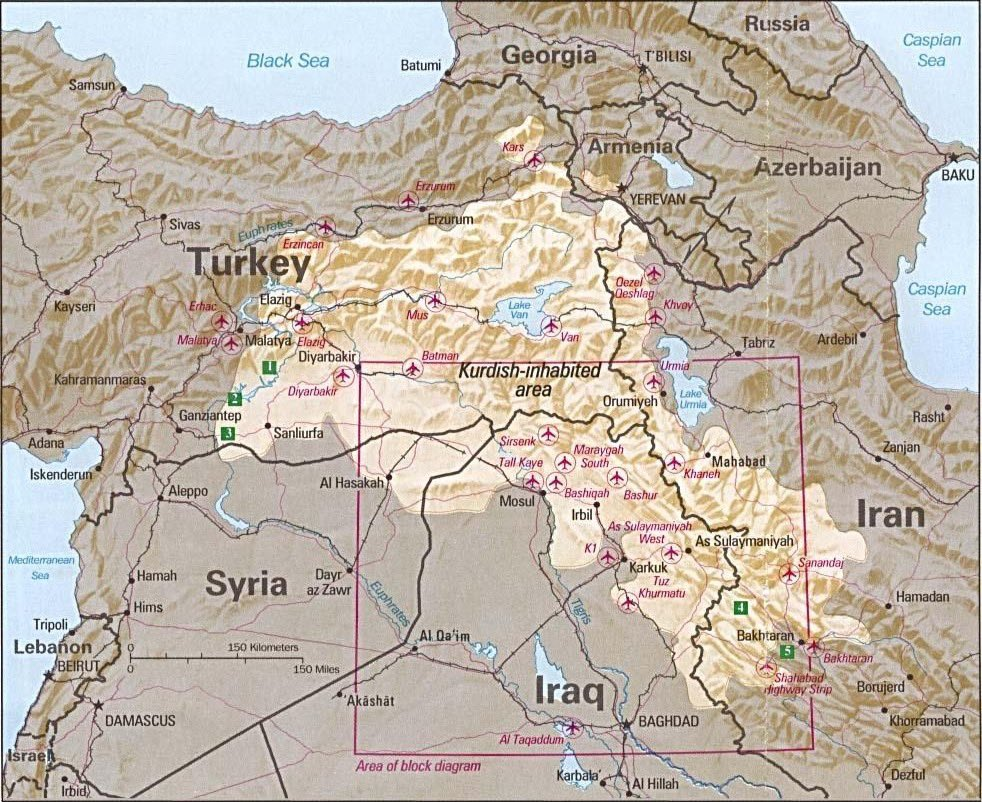
\includegraphics[width=0.8\textwidth]{kurdish.jpeg}
    \caption{库尔德人分布区域} % The caption ends here.
    \small % Apply small font size to the source text.
    \par\vspace{-0.5em} % Add a small vertical space and ensure new paragraph.
    来源: [\url{https://maps.lib.utexas.edu/maps/middle_east_and_asia/kurdish_lands_92.jpg} ]% Source information is now outside the caption.
    \label{fig:kurdish}
\end{figure}

\subsection{政权:政治世界的“操作系统”与“游戏规则”}

我们有了硬件(国家)和灵魂(民族),现在需要一套“操作系统”来决定这台计算机如何运行。这就是“政权”。

\textbf{政权是一套决定权力如何获得、如何行使、以及如何在政府与公民之间分配的根本性规则、规范和制度。} 它回答了最根本的问题:谁有资格统治?通过什么程序上台?权力的界限在哪里?

\begin{itemize}
    \item \textbf{核心比喻:} 政权就是\textbf{政治的“游戏规则”或“操作系统”}。这些规则比任何一届政府都更持久。例如:
    \begin{itemize}
        \item \textbf{民主政权:} 游戏规则是:通过自由、公平、定期的选举来竞争权力。公民享有广泛的权利和自由。这就像一个开源的操作系统,人人都可以参与开发和监督。
        \item \textbf{威权政权:} 游戏规则是:权力集中在少数人或单个政党手中,民众的政治参与受到严格限制。这就像一个封闭的、专有的操作系统,只有特定的“管理员”才有权限。
    \end{itemize}
\end{itemize}
一个国家可以经历政权更迭。例如,1970年代的智利,从民主政权转变为军事独裁政权,再到1990年代回归民主,这期间,“智利”这个国家(State)一直存在,但它的“游戏规则”(Regime)发生了根本性的变化。

\subsection{政府:政治世界的“当班司机”}

最后,我们来到最具体、也最常变动的层面:“政府”。\textbf{政府是当前掌握国家权力、负责日常治理的具体人群。} 他们是“当班的司机”,是操作这台机器的人。

\begin{itemize}
    \item \textbf{核心比喻:} 如果政权是“游戏规则”,那么\textbf{政府就是某一局游戏的“玩家”或“赢家”}。在美国,我们谈论的是“拜登政府”;在英国,是“苏纳克政府”。这些政府通过政权所设定的规则(如选举)上台,他们的任期是有限的。当政府更迭时——比如美国的民主党政府被共和党政府取代——国家的硬件(State)和操作系统(Regime)通常保持不变。
\end{itemize}

\subsection{四位一体:一个实例}

让我们用\textbf{英国}来把这四个概念串起来:

\begin{itemize}
    \item \textbf{国家 (State):} 指的是拥有悠久历史的英国国家机器,包括其常任文官系统、法院、警察和军队。这个“国家”在撒切尔夫人和托尼·布莱尔执政时期都同样存在。
    \item \textbf{民族 (Nation):} 情况复杂。英国国内存在着英格兰、苏格兰、威尔士和北爱尔兰四个不同的民族认同,这正是其政治中持续紧张的来源之一。
    \item \textbf{政权 (Regime):} 是君主立宪制下的议会民主制。这是一套稳定的游戏规则,规定了议会至上、首相由下议院多数党领袖担任等核心原则。
    \item \textbf{政府 (Government):} 指的是当前由保守党组成、由现任首相领导的具体执政团队。这个团队几年后可能会被工党政府所取代。
\end{itemize}

清晰地分辨这四个概念,是进行任何有意义的政治比较的第一步。当我们说“中国很强大”时,我们可能指的是其国家能力(State);当我们讨论“阿拉伯之春”时,我们关注的是政权更迭(Regime Change);当我们听到“特朗普当选”时,我们谈论的是政府轮替(Government)。

\section{选择罗盘:像侦探一样思考}

有了地图,我们还需要罗盘来指导探索。比较政治学不是观点的罗列,而是一门寻求因果解释的科学。为此,学者们主要使用两种互补的研究方法,就像一个破案团队里,既需要深入现场的侦探,也需要分析大数据的犯罪情报官。

\subsection{案例研究:侦探的深度挖掘}

想象一下福尔摩斯接到一个棘手的案子。他会怎么做?他会亲临犯罪现场,仔细勘察每一个细节:地上的烟灰、泥土的痕迹、死者最后的言语。他会深入访谈所有相关人员,试图重构事件发生的完整链条。

\textbf{案例研究就像是侦探的工作。} 它选择一个或少数几个国家(案例),进行深入、细致、长期的考察。研究者可能会学习当地语言,在那个国家生活数年,阅读历史档案,访谈政治人物和普通民众。

\begin{itemize}
    \item \textbf{目标:} 理解特定事件为何以及如何发生,揭示现象背后的复杂因果机制。
    \item \textbf{例子:} 要理解法国大革命为何爆发,一位学者可能会穷尽一生去研究18世纪法国的社会结构、财政状况、启蒙思想和关键人物的决策。
    \item \textbf{优势:} 提供了无与伦比的深度和细节,能够捕捉到宏观数据无法体现的历史背景和文化独特性。
    \item \textbf{劣势:} “以偏概全”的风险。从法国大革命中得出的结论,能用来解释俄国革命吗?我们很难确定一个案例的发现是否具有普遍性。
\end{itemize}

\subsection{统计分析:情报官的宏观扫描}

现在想象一个国家情报机构的分析中心。分析师们不会只盯着一个目标,他们会调动卫星、搜集全球数据,在成千上万的信息点中寻找规律和模式。比如,他们可能会分析数百个军事基地的卫星图像,来判断哪种类型的基地最有可能部署新型武器。

\textbf{统计分析就像是情报官的工作。} 它搜集大量国家(从几十个到上百个)在很长一段时间内的数据,然后运用统计学工具来检验变量之间的相关关系。

\begin{itemize}
    \item \textbf{目标:} 发现跨越国界的、具有普遍性的宏观规律或相关性。
    \item \textbf{例子:} 一位学者想知道经济发展是否促进民主。他会搜集过去50年间全球150个国家的经济数据(如人均GDP)和政治数据(如民主指数),然后用统计软件分析两者之间是否存在显著的正相关。
    \item \textbf{优势:} 覆盖面广,能够识别出个人经验可能忽略的宏大模式,结论具有更强的普遍性。
    \item \textbf{劣势:}
    \begin{enumerate}
        \item \textbf{相关不等于因果:} 统计显示富裕国家大多是民主国家,但这并不能证明是“富裕”导致了“民主”。也可能是民主制度更有利于经济发展,或者存在某个第三方因素同时促进了两者。
        \item \textbf{化约主义风险:} 为了进行量化比较,复杂的现实(如“民主质量”)常常被简化为冷冰冰的数字,忽略了每个国家独特的历史和文化背景。
    \end{enumerate}
\end{itemize}

\subsection{侦探与情报官的联手}

那么,哪种方法更好?这是一个错误的问题。真正优秀的比较政治学研究,会将两者结合起来,让侦探与情报官联手破案。

典型的研究路径是这样的:
\begin{enumerate}
    \item \textbf{情报官先发现模式:} 统计分析发现一个有趣的宏观规律,例如,“依赖石油出口的威权国家,似乎比其他威权国家更难实现民主化转型。”
    \item \textbf{侦探再深入调查:} 接着,研究者会选择几个典型的“石油国家”(如沙特阿拉伯、委内瑞拉)和非典型的案例(如成功转型的挪威)进行深入的案例研究。他要去现场探究,石油财富到底是如何通过具体的机制(例如,政府用石油收入收买民众、豢养庞大的安全部队、免除税收从而削弱公民的问责要求)来阻碍民主化的。
\end{enumerate}

通过这种方式,统计分析的广度与案例研究的深度实现了完美的互补。我们既看到了森林,也看清了树木。

\section*{本章小结}
\addcontentsline{toc}{section}{本章小结}

现在,你的探险行囊里已经装上了最基础的装备。你有了\textbf{一张地图},懂得如何区分国家(硬件)、民族(灵魂)、政权(操作系统)和政府(当班司机)这四个核心地标。你也有了\textbf{一支罗盘},知道可以通过侦探式的案例研究和情报官式的统计分析,来探索政治世界的奥秘。

你已经准备好成为一名敏锐的观察者和思考者。在接下来的章节中,我们将手持地图与罗盘,正式踏入政治世界的腹地,去探索那些最棘手、也最迷人的“大问题”——国家为何强大或脆弱?民主为何兴盛又衰退?威权统治者有哪些不为人知的生存秘诀?让我们一同启程,去比较、去发现、去理解。

\part{大问题:国家、政体与冲突}

\chapter{国家是如何炼成的?——从战争机器到“守夜人”}

在第一章中,我们为政治世界的探险之旅备齐了“地图”与“罗盘”,厘清了“国家”、“政权”等核心概念。现在,我们将正式踏入这片广袤大陆的腹地,首先聚焦于其中最基础、也最强大的存在——国家。想象一下,你手中的护照、钱包里的身份证、缴纳税款的通知单,甚至是你脚下平整的公路和头顶明亮的街灯——这些我们习以为常的事物,背后都站着一个巨大而无形的存在:\textbf{国家(The State)}。它既是我们安全的保障,又是我们自由的约束;它能像新加坡一样创造经济奇迹,也能像索马里一样陷入无尽的混乱。

这个在我们的生活中无处不在、拥有至高权力的“利维坦”,究竟从何而来?它不是从天而降,更不是温情脉脉的田园诗。在很大程度上,现代国家的诞生,浸透着鲜血与炮火。

\section{“战争制造国家,国家发动战争”:欧洲的血腥往事}

让我们把时钟拨回到中世纪晚期的欧洲。那时的欧洲大陆,根本不存在我们今天所熟知的、有着清晰边界和统一法律的国家。它更像一盘散沙,遍布着上千个大大小小的政治单元:国王、封建领主、主教、城邦、部落联盟……他们彼此征伐不休,权力犬牙交错。如果你是一个生活在那个时代的君主,你每天醒来思考的头等大事只有一个:\textbf{生存}。

如何生存?答案简单而残酷:发动战争,消灭或吞并你的邻居,否则你就会被他们消灭。著名的历史社会学家查尔斯·蒂利(Charles Tilly)用一句冷酷而精辟的话总结了这一过程:“\textbf{战争制造国家,国家发动战争(War made the state, and the state made war)。}”

这听起来像一个黑帮的“保护费”生意,事实也相差无几。让我们拆解这个“暴力驱动”的逻辑链:

\begin{enumerate}
    \item \textbf{战争的驱动}:为了在残酷的竞争中胜出,统治者需要一支更强大、更专业的军队。这需要钱,大量的钱,来购买武器、支付军饷。
    \item \textbf{榨取资源的需要(Extraction)}:钱从哪里来?最稳定可靠的方式就是向其治下的民众\textbf{征税}。为了有效征税,统治者不能再像过去那样依赖松散的封建贵族。他必须建立一个\textbf{中央集权的官僚体系}——税务官、会计、书记员——直接深入到社会的毛细血管,去统计人口、丈量土地、收取金钱。现代国家的财政部和税务局的雏形,就这样在战争的催逼下诞生了。
    \item \textbf{控制内部的需要(Coercion)}:民众凭什么乖乖交税?凭什么应征入伍?因为统治者垄断了暴力。他必须建立一支\textbf{警察部队},收缴民间武器,镇压内部反抗,确保税收和兵源。通过将暴力工具(军队、警察)牢牢掌握在自己手中,统治者实现了\textbf{暴力的垄断},这是国家主权最核心的特征。
    \item \textbf{资本的助力(Capital)}:光靠税收往往还不够。统治者还需要向富有的商人和银行家借贷。为了让他们愿意借钱,统治者必须保护私有产权,建立可信的法律和法庭体系,以确保契约能够履行。于是,现代的金融和司法体系也开始萌芽。
\end{enumerate}

这个过程是一个自我强化的循环:更强的征税能力和暴力垄断,意味着能供养更强的军队;更强的军队,意味着能打赢更多战争,占领更多土地,从而获得更多税基和资源。数百年间,欧洲大陆上那些无力建立高效官僚体系、无法垄断暴力的弱小政治体,都在这场残酷的“大逃杀”中被淘汰。最终,从一片混乱中崛起的,是少数几个拥有强大中央政府、明确领土边界和高效汲取能力的幸存者——也就是我们今天所知的法国、英国、西班牙等现代民族国家。

所以,现代国家的诞生,并非源于某个哲学家在书斋里的崇高设计,而是暴力竞争的意外产物。它是一个从“有组织的暴力团伙”演变而来的“制度化的保护费集团”。

\section{镜鉴:中国的历史回响——另一条炼成之路}

蒂利的理论如同一把解剖刀,精准地剖开了欧洲国家形成的肌理。然而,将目光投向东方,我们会发现一幅截然不同、却同样波澜壮阔的国家形成图景。中国的历史,为我们提供了“战争制造国家”理论的一个重要参照与补充。

与中世纪晚期欧洲的“千国林立”不同,一个统一的、中央集权的官僚帝国在中国出现得非常早。早在公元前3世纪,秦始皇就已通过战争统一了六国,建立了“车同轨,书同文”的庞大帝国。从那时起,中国历史的主旋律,就不再是欧洲那种数百个政治实体之间残酷的“大逃杀”,而是如何维持和重建一个已经存在的、广土众民的统一国家。

这就导致了国家面临的核心挑战截然不同:

\begin{itemize}
    \item \textbf{威胁来源不同:} 欧洲国家主要面对的是来自邻国的、旗鼓相当的外部竞争。而中华帝国在大部分时间里,其心腹大患是两个:其一是周期性的、大规模的内部农民起义,其二是来自北方草原的游牧民族入侵。
    \item \textbf{锻造机制不同:} 为了应对这些挑战,中华帝国发展出了一套独特的国家锻造机制。它不完全依赖于蒂利所说的“战争-榨取”循环。为了维持内部稳定,它需要建立一个能深入到县乡层级的庞大文官官僚体系,通过科举制度选拔非世袭的、忠于中央的知识精英来治理国家。为了传播统一的价值观、降低治理成本,它高度依赖儒家意识形态的教化作用。这些,都是欧洲早期国家所不具备的。
\end{itemize}

因此,如果说欧洲国家是在持续不断的外部战争“高压锅”中被锻造出来的“精炼钢”,那么中华帝国则更像是在应对内部离心力和外部冲击的反复“淬火”中形成的、具有强大“修复”能力的“记忆合金”。它的历史呈现出一种独特的“王朝循环”:统一、鼎盛、衰败、分裂,再到新的统一。国家的“硬件”(官僚体制)和“软件”(大一统思想)在王朝更迭中被反复摧毁和重建,但其核心模式却表现出惊人的连续性。

中国的案例告诉我们,蒂利的理论并非放之四海而皆准的普世定律,而是一个极其深刻的“欧洲特殊论”。国家形成的路径不止一条。面对不同类型的生存威胁,统治者会发展出迥异的制度安排和统治策略。这也为我们接下来要探讨的问题——当代国家的强弱之分——提供了更广阔的比较视野。

\section{前沿视角:为何有些国家强大,有些国家脆弱?}

欧洲的这套“战争-锻造”模式,与中国的“王朝循环”经验,共同为我们理解国家的起源提供了深刻的洞见。但这两种古典剧本,似乎都难以完全解释当今世界的图景。许多在二战后独立的亚非拉国家,并没有经历欧洲那样长达数百年的内部战争整合,也没有中国那样悠久的帝国传承。它们的边界往往是殖民者在地图上随手划定的,其国家机器也是从殖民者手中仓促继承的。它们“生而为国”,却未经“炼成”。

这就引出了当今比较政治学最核心的问题:为什么有些国家,如高效廉洁的新加坡,能实现惊人的发展与稳定;而另一些国家,如陷入内战泥潭的索马里,连最基本的社会秩序都无法维持?

答案的关键在于两个概念:\textbf{国家能力(State Capacity)}和\textbf{合法性(Legitimacy)}。

\subsection{国家能力:国家这台“机器”的性能如何?}

“国家能力”指的是一个国家将其意志转化为行动、有效治理其领土和民众的实际本领。它就像一台电脑的硬件和操作系统,决定了国家这台“机器”的性能。一个高能力的国家,至少能在以下几个方面做得很好:
\begin{itemize}
    \item \textbf{汲取能力}:能够有效地从社会中征收税收,为国家运转提供燃料。
    \item \textbf{强制能力}:能够垄断暴力,维持国内秩序,保卫国家边境。
    \item \textbf{规管能力}:能够制定和执行法律法规,管理市场,保护环境。
    \item \textbf{供给能力}:能够提供公共产品和服务,如基础设施(道路、网络)、教育和公共卫生。
\end{itemize}

以\textbf{新加坡}为例,它被誉为“高能力国家”的典范。其政府拥有一支专业、廉洁、高效的精英官僚队伍,能够制定并执行长远的国家发展战略;其税收体系公平高效,为世界一流的基础设施和公共服务提供了充足财源;其法律体系严格而透明,确保了社会的高度稳定和商业的繁荣。

反观\textbf{索马里},它是一个典型的“脆弱国家”(Fragile State),甚至被称为“失败国家”(Failed State)。其中央政府的政令不出首都摩加迪沙,无法在全国范围内征税,无法提供任何有效的公共服务,更无法垄断暴力——各路军阀、部落武装和极端组织割据一方,国家的“硬件”和“操作系统”几乎全面崩溃。

\subsection{合法性:民众为何会服从?}

如果说“国家能力”是国家的“手脚”,那么“合法性”就是国家的“灵魂”。合法性,指的是民众发自内心地认可国家的统治权,认为国家的权威是正当的、应当被服从的。这种服从,并非仅仅出于对惩罚的恐惧。

德国社会学家马克斯·韦伯(Max Weber)曾指出合法性的三种来源:
\begin{itemize}
    \item \textbf{传统型合法性}:源于“历来如此”的习俗和传统,如世袭的君主制。
    \item \textbf{魅力型(克里斯玛型)合法性}:源于领袖非凡的个人魅力和感召力,如革命领袖。
    \item \textbf{法理型合法性}:源于对法律和制度本身的信任。人们服从的不是某个具体的人,而是相信这些规则和程序是公平、公正的。这是现代国家最稳定、最重要的合法性基础。
\end{itemize}

\textbf{国家能力与合法性,是一对共生共荣的孪生兄弟。} 一个高能力的国家,可以通过提供良好的公共服务和安全保障来赢得民众的认可,从而增强其合法性。而一个拥有高度合法性的国家,民众更愿意自觉遵守法律、缴纳税款,这反过来又极大地提升了国家的治理能力。

反之,一个低能力的国家,无法保护人民、提供福利,其合法性就会不断流失。而合法性的丧失,又会导致民众抗税、反抗,使国家能力雪上加霜,陷入“低能力-低合法性”的恶性循环,最终走向脆弱甚至崩溃。

\section{从“战争机器”到“守夜人”再到更多}

我们看到,国家从一个为战争而生的暴力机器,逐渐演化。随着其能力和合法性的巩固,社会对它的期望也在不断变化。

在19世纪的古典自由主义者看来,最理想的国家是\textbf{“守夜人国家”(Night-watchman State)}。它的职能应该被限制在最小范围:像一个守夜人一样,只负责保护公民的人身和财产安全,维护契约的履行,除此之外,不应干涉经济和个人生活。

然而,20世纪的两次世界大战和大萧条,彻底改变了人们的看法。民众开始要求国家提供更多保障,于是\textbf{“福利国家”(Welfare State)}应运而生,国家开始承担起教育、医疗、养老、失业救济等广泛的社会责任。而在东亚,一些国家更是扮演了\textbf{“发展型国家”(Developmental State)}的角色,深度介入和引导经济发展,创造了举世瞩目的经济奇迹。(我们将在后续章节深入探讨这些模式)

\section*{结语}
\addcontentsline{toc}{section}{结语}

回顾国家“炼成”的旅程,我们看到,它既有血腥暴力的起源,也有迈向文明与服务的演进。理解这段历史,我们才能明白,一个强大而负责任的国家并非理所当然。它是历史的产物,需要“能力”与“合法性”两大支柱的精心维护。

通过比较欧洲历史上的“战争锻造”与当代发展中国家的“国家建构”,通过审视新加坡的成功与索马里的困境,我们得以窥见国家命运的分野所在。而下一个更令人着迷的问题是:当国家这台机器被锻造出来后,它应该由谁来掌控?如何掌控?这就是我们将要进入的下一个世界——民主与威权的激烈交锋。

\chapter{民主的浪潮与暗礁——为何有些民主“活下来了”,有些却“死去了”?}

在上一章中,我们深入探讨了国家的起源与形成,理解了国家能力和合法性如何决定一个国家的强弱。现在,我们将目光转向国家权力如何被组织和行使的核心问题。20世纪末的空气中弥漫着一种历史性的乐观情绪。1989年,柏林墙在万众欢呼中倒塌;随后,东欧的卫星国纷纷挣脱苏联的引力,投向民主的怀抱。弗朗西斯·福山甚至大胆宣告,我们可能正见证着“历史的终结”——自由民主制作为人类政府的最终形式,已经取得了决定性的胜利。这股浪潮是如此汹涌,以至于人们普遍相信,民主不仅是最好的制度,也是最不可避免的归宿。

然而,三十年后的今天,当初的乐观早已被一种深刻的焦虑所取代。曾经的民主“模范生”如匈牙利和土耳其,正一步步滑向威权的深渊;即便是最老牌的民主国家如美国,也出现了令人不安的制度侵蚀迹象。民主的航船似乎驶离了开阔的蓝海,闯入了一片遍布暗礁的危险水域。

这不禁让我们提出本章的核心问题:民主的扩张背后究竟是什么力量在推动?而今天,又是什么样的暗礁,使得一些民主政体搁浅、沉没,甚至被曾经的舵手亲手凿穿?为何有些民主能够经受住风暴的考验,而另一些则脆弱不堪,迅速“死去”?

\section{宏大叙事:席卷全球的民主化浪潮}

要理解今天的困境,我们必须先回顾昨天的辉煌。已故的哈佛大学政治学家塞缪尔·亨廷顿(Samuel Huntington)曾用一个极具影响力的比喻,将全球民主化的进程描述为三波巨大的“浪潮”。

\begin{itemize}
    \item \textbf{第一波浪潮(19世纪初至1920年代):} 这是一次漫长而缓慢的浪潮,发源于西欧和北美。美国革命和法国大革命的理念,如同投入世界政治池塘的第一颗石子,激起的涟漪逐渐扩展。选举权在这些国家缓慢扩大,议会的权力得到巩固。然而,这波浪潮在两次世界大战之间遭遇了强劲的“回头浪”,法西斯主义、纳粹主义和共产主义的崛起,让许多新兴的民主政体夭折。
    \item \textbf{第二波浪潮(二战后至1960年代初):} 第二次世界大战的结束,为民主带来了新的机遇。在盟军的占领和扶持下,德国、意大利、日本等前轴心国成功实现了民主转型。同时,亚非拉地区的非殖民化运动也催生了一批新兴独立国家,它们大多在独立之初采纳了民主宪法,比如印度——这个世界上人口最多的民主国家。但这波浪潮同样短暂,1960年代和1970年代,许多新兴民主国家在经济困境和政治动荡中,纷纷被军事政变推翻,再次陷入威权统治的“回头浪”。
    \item \textbf{第三波浪潮(1974年至今):} 这是迄今为止规模最大、影响最深远的一波浪潮。它始于南欧的边缘:1974年葡萄牙的“康乃馨革命”终结了数十年的独裁统治。随后,西班牙和希腊也成功转型。浪潮接着席卷拉丁美洲,阿根廷、巴西、智利的军政府相继倒台。而这波浪潮的最高峰,无疑是1989-1991年苏联集团的崩溃,它戏剧性地为全球民主版图增添了数十个新成员。
\end{itemize}

\begin{figure}[htbp]
    \centering
    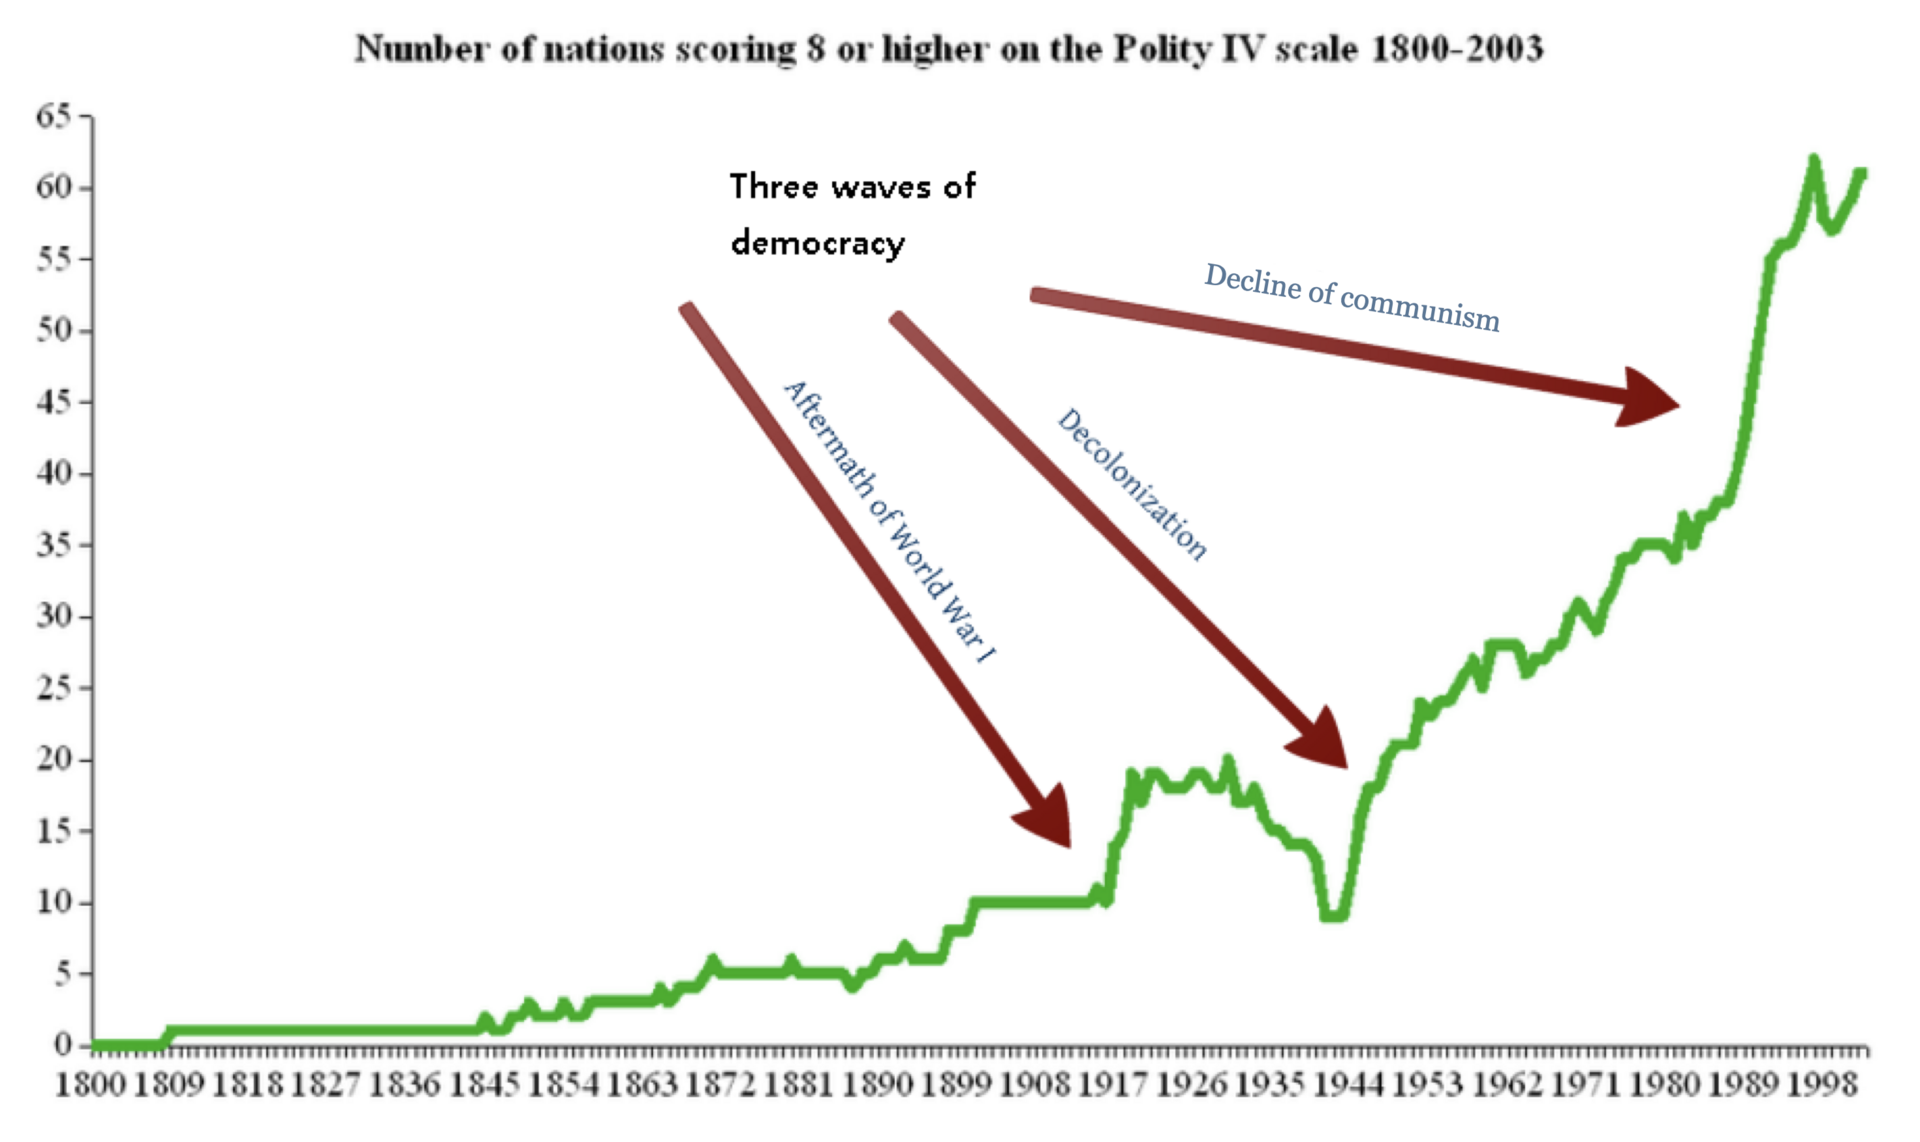
\includegraphics[width=\textwidth]{Waves_of_democracy.png} % Assuming you have an image file named democracy_waves.png
    \caption{全球民主化浪潮}
    \small
    来源: [\url{https://upload.wikimedia.org/wikipedia/commons/e/e6/Waves_of_democracy.png}]
    \label{fig:democracy_waves}
\end{figure}


是什么驱动了这排山倒海般的浪潮?学者们发现了几个关键的驱动引擎:
\begin{enumerate}
    \item \textbf{经济发展与中产阶级的崛起:} 这是最经典的解释,即“现代化理论”。其核心逻辑是:当一个国家变得更富裕,工业化和城市化水平提高,教育普及,一个庞大、独立且受过良好教育的中产阶级便会应运而生。这些人有资产、有知识、有闲暇,他们更关心自己的权利,看重法治对财产权的保护,并且不能容忍政府的专断和腐败。正如政治学家西摩·马丁·李普塞特(Seymour Martin Lipset)所言:“一个国家越是富裕,其维持民主的机会就越大。”一个温饱都成问题的赤贫社会,很难孕育出稳定的民主;反之,一个富裕的中产社会,是民主最坚实的土壤。

    然而,这一理论并非无懈可击的“铁律”。比较的视野很快让我们看到了它的局限性。一方面,世界上存在大量富裕的威权国家,尤其是那些依赖石油出口的“寻租国家”(Rentier States)。在这些国家(如沙特阿拉伯),巨额的石油财富由国家直接掌控,政府无需通过向民众征税来维持运转,反而可以用福利收买民众,并建立强大的镇压机器。财富没有催生出独立的、要求政治权利的中产阶级,反而巩固了威权统治。另一方面,像印度这样的国家,尽管在独立后很长一段时间里经济相对落后,却奇迹般地维持了稳定的民主制度。这表明,单纯的经济水平无法解释一切。印度的案例迫使我们将目光投向其他因素:其从英国继承的制度遗产、国大党精英对民主的承诺,以及活跃的公民社会。

    因此,现代化理论虽然揭示了经济发展与民主之间重要的相关性,但它并非一个决定性的预言。这些重要的“例外”提醒我们,民主的发生与巩固,是一场由经济、文化、制度和国际环境等多种力量共同谱写的复杂戏剧。

    \item \textbf{国际环境的变迁:} 政治转型从不是一个孤立的国内事件。在第三波浪潮中,外部力量扮演了至关重要的角色。首先是西方民主国家(尤其是美国)的政策,它们通过外交压力、经济援助甚至军事干预来推动民主。其次是苏联的衰落和解体,这让全球许多依赖苏联支持的左翼独裁政权失去了靠山,也让它们失去了与西方民主竞争的意识形态合法性。最后是“滚雪球效应”或“示范效应”:当一个国家的民主转型成功后,其邻国的人民和精英会备受鼓舞,意识到“改变是可能的”,从而引发区域性的连锁反应。波兰的团结工会运动,无疑激励了匈牙利和捷克斯洛伐克的民主派。

    \item \textbf{观念的转变与公民文化的成熟:} 民主不仅是一套制度,更是一种深入人心的信念。随着全球化的加深,关于人权、自由和政府问责的观念,通过教育、媒体和人员往来,传播到世界的各个角落。天主教会从支持威权(如在拉丁美洲)转向倡导人权,就是一个重要的观念转变。这种自下而上的文化变迁,为民主转型提供了深厚的社会基础。
\end{enumerate}
这三大引擎共同作用,造就了20世纪末民主的辉煌。然而,正如每一波浪潮之后都可能出现“回头浪”一样,第三波浪潮的洪峰过后,我们看到的不是风平浪静,而是危险的暗礁。

\section{前沿辩论:民主如何“合法地”死去?}

今天,对民主最大的威胁,不再是上个世纪那种明目张胆的军事政变——坦克开上街头,将军发表电视讲话,宣布解散国会。哈佛大学的政治学家史蒂文·列维茨基(Steven Levitsky)和丹尼尔·齐布拉特(Daniel Ziblatt)在他们的著作《民主如何消亡》(\textit{How Democracies Die})中指出,当代民主的死亡方式发生了根本性的变化。它不再是一场猝死,而更像是一场慢性病。

这种新的死亡方式,我们称之为\textbf{“民主倒退”(Democratic Backsliding)}。

它指的是一个由民选领导人领导的、循序渐进的、通常是披着合法外衣的侵蚀民主制度和规范的过程。这些领导人不是通过暴力革命上台,而是在选民的欢呼声中赢得选举。然而,一旦大权在握,他们便开始系统性地、一步步地拆解民主的防御工事。这个过程就像“温水煮青蛙”,每一次的改变或许都看似微小且合法,但日积月累,最终会从根本上改变政体的性质。

让我们以匈牙利和土耳其这两个最典型的案例,来解剖民主倒退的“操作手册”:

\textbf{第一步:攻占“裁判席”——控制司法与中立机构。}
民主的基石之一是中立的裁判,包括独立的法院、选举委员会、审计机构等。民选的威权倾向者上台后,首要目标就是将这些裁判换成自己的“自己人”。在匈牙利,总理欧尔班领导的青民盟利用其在国会的绝对多数,强行修改宪法,降低了宪法法院法官的退休年龄,从而得以安插大量忠于自己的法官,并极大地削弱了宪法法院的审查权。在土耳其,总统埃尔多安在2016年未遂政变后,以清洗“政变分子”为名,解雇了数千名法官和检察官,将司法系统牢牢掌握在自己手中。当裁判不再中立,比赛的公平性便无从谈起。

\textbf{第二步:压制对手——削弱政治反对派和公民社会。}
他们不会直接取缔反对党,而是利用手中的国家机器,让对手的生存空间越来越小。这包括:通过税收、监管等手段骚扰反对派金主的企业;操控国有媒体,让反对派的声音无法有效传播;甚至以“反腐”、“叛国”等名义对政治对手进行司法追诉。在土耳其,许多反对派议员和市长被剥夺职位甚至投入监狱。在匈牙利,与欧尔班不睦的媒体和非政府组织(NGOs)则被贴上“外国代理人”的标签,受到严格限制。

\textbf{第三步:重划“游戏规则”——操纵选举和媒体环境。}
这是最精巧的一步。他们不会取消选举,反而会更加“热衷”于选举,但他们会确保游戏规则对自己绝对有利。最常见的手段是“杰利蝾螈”(Gerrymandering),即以一种极为不公平的方式重划选区,使得执政党可以用较少的选票赢得更多的席位。匈牙利青民盟正是通过一套精心设计的选举法,确保了自己即便在支持率下降的情况下,也能在国会中占据压倒性优势。同时,他们通过收购、扶持亲政府媒体、打压独立媒体,建立起一个巨大的宣传机器,让选民难以接触到真实、多元的信息。

值得警惕的是,这种民主倒退的症状,甚至在一些最成熟的民主国家也若隐若现。例如在美国,近年来出现的对选举结果公正性的反复攻击、将新闻媒体斥为“人民的公敌”、以及对司法独立性的公开施压,都触碰了民主制度赖以生存的“软性护栏”——即那些不成文的政治规范,如对竞争对手的相互容忍和对制度的尊重。

\section{民主的暗礁:我们为何走到了今天?}

为何在21世纪,民主的航船会如此轻易地撞上这些暗礁?这背后是更深层次的经济、文化和技术变革。

\begin{enumerate}
    \item \textbf{经济的焦虑与不平等:} 全球化和自动化在创造巨大财富的同时,也在发达国家内部制造了大量的“失败者”。当传统制造业岗位流失,蓝领工薪阶层的生活水平停滞不前甚至下降时,他们感到被精英阶层背叛和抛弃。这种普遍的经济焦虑,为那些承诺“夺回控制权”、将问题归咎于移民和外国的民粹主义领导人提供了沃土。
    \item \textbf{文化的裂痕与身份政治:} 与经济焦虑并行的,是深刻的文化反弹。在全球化带来的多元文化和进步主义价值观(如女权、LGBTQ+权利)面前,社会中相当一部分保守群体感到自己的生活方式和传统价值受到了威胁。这种文化上的不安全感,使得“我们”与“他们”的身份认同变得异常尖锐。政治不再是关于政策的理性辩论,而变成了捍卫自身文化和身份的“部落战争”。在这种氛围下,人们更容易追随那些承诺捍卫“我们”身份认同的强人领袖。
    \item \textbf{信息生态的剧变:} 社交媒体的崛起,彻底改变了我们获取信息和参与政治的方式。它打破了传统媒体的权威,但也创造了大量的“回音室”和“过滤泡”,使得谎言和阴谋论以前所未有的速度传播。算法推荐将我们推向更极端的内容,加剧了政治极化。当人们生活在完全不同的事实宇宙中,将对方视为无知、邪恶的敌人时,民主所必需的妥协与共识便荡然无存。
\end{enumerate}

\section*{结语:在分裂的世界里重新守护民主}
\addcontentsline{toc}{section}{结语:在分裂的世界里重新守护民主}

回顾民主的百年历程,我们看到它既有波澜壮阔的胜利,也面临着阴险致命的挑战。民主从来不是历史的必然,它更像是一座需要持续维护和加固的精巧建筑。

今天的民主保卫战,战场已经改变。它不再仅仅是在广场上对抗坦克,更是在法庭里捍卫司法独立,在议会中守护公平的议事规则,在社交媒体上辨别真伪信息,以及最关键的——在每一次投票中,做出审慎的选择。

理解当代民主“死亡”的新方式,看清那些以“人民”之名、行侵蚀民主之实的“合法”手段,是我们这个时代每个公民的必修课。因为只有看清了那些水面之下的暗礁,我们才有可能驾驶民主的航船,绕开险滩,继续前行。这场关乎我们共同命运的航行,远未结束。

\chapter{威权者的“生存游戏”——揭秘现代独裁的运作密码}

在上一章中,我们探讨了民主的兴衰与挑战,特别是民选领导人如何“合法地”侵蚀民主。然而,在世界政治的版图上,威权主义依然占据着重要一席。当我们想到“独裁”,脑海中浮现的或许是旧时代的刻板印象:一个戴着墨镜、身着军装的将军在阳台上咆哮,背后是成排的坦克和噤若寒蝉的民众。这种赤裸裸的暴力统治,确实是威权主义的一种形态。然而,在21世纪,这场“游戏”的玩法已经变得远为复杂和精致。

现代威权者们更像是一位精明的CEO、一位高超的魔术师和一位冷酷的棋手。他们深知,仅靠恐惧来维持的统治是脆弱且昂贵的。因此,他们发展出了一套复杂的生存工具箱,其目的不仅是压制反对,更是要塑造一个让其统治显得“理所当然”甚至“不可或缺”的政治环境。本章将带领读者走进威权主义的幕后,揭示这场精密“生存游戏”的规则与策略。

\section{打破刻板印象:威权主义并非铁板一块}

首先,我们必须抛弃将所有非民主国家都视为一个模样的简单看法。事实上,威权政体内部的多样性,可能比民主国家之间的差异还要大。了解它们的类型,是理解其行为逻辑的第一步。我们可以将它们粗略地归入一个“威权动物园”,其中最主要的三种类型是:

\subsection{个人独裁:权力系于一人之身}

这是我们最熟悉的独裁形态,整个国家的命运与一个人的意志、健康甚至情绪紧密相连。从土库曼斯坦那位为自己和家人建造黄金雕像的“土库曼巴希”,到朝鲜的金氏家族,个人独裁的特点是权力高度集中,制度化程度极低。
\begin{itemize}
    \item \textbf{优势:} 决策效率极高(因为无人敢于反对),能够迅速动员资源执行独裁者的意志。
    \item \textbf{弱点:} 极端不稳定和脆弱。它的最大风险在于 \textbf{“继承危机”}。一旦强人离世或失势,整个权力结构可能瞬间崩塌,因为没有任何制度化的规则来决定谁是下一个掌权者,极易引发血腥的内部斗争。同时,由于决策仅凭一人好恶,往往会导致灾难性的政策错误。
\end{itemize}

\subsection{军事强权:枪杆子里出政权}

在这种政体中,统治者是一群来自军队的高级军官。他们通常通过政变上台,承诺恢复“秩序与稳定”。近年的缅甸、历史上的智利(皮诺切特时期)和阿根廷军政府都是典型例子。
\begin{itemize}
    \item \textbf{优势:} 拥有无可匹敌的暴力机器和组织纪律,能够有效镇压反对派,强制推行政策。
    \item \textbf{弱点:} \textbf{缺乏统治的合法性基础}。军人被认为是保家卫国的,而非治理国家的。因此,军事政权常常面临“为何是你们在统治”的灵魂拷问。他们往往是过渡性的,在完成其“历史使命”(如清除异己、稳定局势)后,可能会选择“还政于民”,当然,是在一个确保其自身利益不受侵犯的新政治框架下。
\end{itemize}

\subsection{一党专政:最坚韧的“利维坦”}

这是迄今为止最稳定、最持久的威权模式。在这种模式下,权力不属于某个人或某个小团体,而是被一个庞大的、制度化的执政党所垄断。从中国的共产党到越南的共产党,再到曾经的新加坡人民行动党(在功能上),一党制展现出惊人的韧性。
\begin{itemize}
    \item \textbf{优势:} 它解决了个人独裁和军事强权的致命弱点。通过党内制度,它 \textbf{解决了继承问题}(如设立任期限制、隔代指定接班人等),避免了权力真空。它能够广泛吸纳社会精英,将其整合进体制内,并通过庞大的组织网络渗透到社会的每一个角落,实现对国家的深度控制。
    \item \textbf{弱点:} 容易变得官僚化、僵化和腐败。由于缺乏外部监督,党内的纪律和自我革新能力成为其能否长期维持活力的关键。一旦党开始脱离民众、腐败滋生,其统治基础同样会受到侵蚀。
\end{itemize}

理解这三种类型的区别至关重要。一个个人独裁者可能会因为一次中风而导致国家动荡,而一个一党制国家则可能在领袖去世后平稳过渡。它们的优势和软肋,决定了它们会采取何种策略来玩好这场“生存游戏”。

\section{现代独裁的运作密码:不止于暴力镇压}

如果说识别不同类型的威权政体是第一步,那么解密它们共同的、日益复杂的统治术,则是看懂现代政治的关键。现代威权者们知道,铁拳虽硬,但若能戴上一只“天鹅绒手套”,效果会更好。

\subsection{选举式威权主义:一场精心编排的“民主秀”}

这是当今最流行的一种威权伪装。这些政权定期举行选举,甚至允许反对党存在,但整个竞争环境被高度操控,以确保执政者永远不会输。俄罗斯、匈牙利、土耳其等国都是此中高手。他们为何要费力上演这出戏?
\begin{itemize}
    \item \textbf{制造合法性假象:} 对内,选举可以营造出一种“人民授权”的表象,安抚部分民众;对外,它可以应付国际社会的批评,让政权看起来更像一个“正常国家”。
    \item \textbf{收集信息与分化对手:} 选举像一次“政治普查”,让统治者知道哪些地区的支持率低,需要加强控制。同时,允许一些弱小的反对党存在,可以分化反对派阵营,避免他们团结成一股强大的力量。
    \item \textbf{手段:} 他们操控选举的方式包括:控制绝大多数媒体,抹黑或 disqualify 有威胁的反对派候选人,利用国家资源进行竞选宣传,以及在投票和计票环节进行微妙的舞弊。
\end{itemize}

\subsection{精密的信息控制:从“防火墙”到“舆论洪水”}

旧式独裁满足于封锁信息,而新式独裁则致力于塑造信息。它们意识到,在一个信息爆炸的时代,简单的封禁是无效的。
\begin{itemize}
    \item \textbf{“防火墙”与审查 (Censorship):} 这是基础操作。通过技术手段(如中国的“防火长城”)屏蔽境外敏感信息,通过人工审查删除国内网络上的负面言论。
    \item \textbf{“舆论洪水”与引导 (Flooding \& Propaganda 2.0):} 这才是更高明的策略。与其费力删除一条负面帖子,不如用成千上万条正面或无关信息将其淹没。政府雇佣大量网评员(俗称“五毛党”或“水军”),在社交媒体上制造支持政府的声浪,转移公众对敏感议题的注意力。它们不再仅仅是说“我们是伟大的”,而是通过弘扬民族主义、宣传生活美好、挑起社会内部矛盾等方式,让批评政府的声音变得微不足道或不合时宜。
\end{itemize}

\subsection{精英笼络:把潜在的敌人变成“自己人”}

聪明的威权者明白,最危险的敌人往往来自内部。因此,与其将所有精英都视为潜在威胁,不如将他们吸纳进体制,让他们成为既得利益者。
\begin{itemize}
    \item \textbf{如何笼络?} 方式多种多样。可以是在名义上的议会或政治协商机构中给他们一个席位,让他们有参政的“荣誉感”;可以是给予他们商业上的特许经营权,让他们发家致富,从而将自己的经济利益与政权的稳定捆绑在一起;还可以是将他们的子女送入最好的学校,或提拔到政府的关键岗位。通过这种方式,统治者编织了一张巨大的利益网络,让精英阶层认识到:支持政权,荣华富贵;反对政权,一无所有。
\end{itemize}

\subsection{绩效合法性:“面包”换“选票”的隐性契约}

这是许多威权政体,尤其是东亚一些国家和地区,最重要的合法性来源。其核心是一种与民众的隐性社会契约:“\textbf{我们(政府)为你们提供经济高速增长、社会稳定和国家荣耀,而你们(民众)则不要过问政治、挑战我们的统治权。}”
\begin{itemize}
    \item \textbf{以中国为例:} 过去几十年惊人的经济发展,让亿万人民摆脱贫困,生活水平显著提高。这种实实在在的物质改善,为执政党赢得了巨大的民众支持,远比任何政治宣传都有效。这种“办实事”的能力,使其统治在许多人眼中具有了强大的“绩效合法性”。
    \item \textbf{脆弱的根基:} 然而,这种合法性也是一把双刃剑。它把政权的命运和经济表现紧紧地绑在了一起。一旦经济增长放缓、失业率上升、社会问题凸显,民众对政府的满意度就可能迅速下降。当“面包”不再充足时,人们就可能会开始想要“选票”了。届时,政权将面临严峻的考验。
\end{itemize}

\section*{结语:一场没有终局的博弈}
\addcontentsline{toc}{section}{结语:一场没有终局的博弈}

威权主义远非一个行将就木的过时产物。它在21世纪展现出了惊人的适应力和创新能力,演变成了一套复杂的、多层次的统治系统。它用选举的仪式模糊独裁的实质,用信息的洪水冲淡异见的声响,用利益的糖衣腐蚀反抗的意志,用经济的成就换取民众的默许。

理解这些精密的“生存游戏”规则,我们才能穿透表象,看清这些政权运作的真实逻辑。我们才能明白,为何在一些国家,经济繁荣却并未带来民主;为何一些看似拥有选举的“民主国家”,其自由内核却在被逐渐掏空。这场威权者与社会力量之间的博弈,是一场动态的、没有终局的较量。而当这场“游戏”的规则被打破,当笼络与收买不再有效时,暴力与冲突的幽灵,就可能再次登场——这正是我们下一章将要探讨的主题。

\chapter{枪声与怒火——我们如何理解政治暴力?}

在前面的章节中,我们探讨了民主与威权政体的运作逻辑。然而,无论是民主还是威权,当政治秩序失灵,社会矛盾激化到无法通过现有规则解决时,我们往往会看到最令人心碎的景象——政治暴力。当电视新闻的画面被熊熊燃烧的建筑、街头愤怒的抗议者和荷枪实弹的士兵所占据,当“内战”、“革命”或“恐怖袭击”这些词语冲击着我们的耳膜时,一种简单而直观的解释会迅速浮现在我们的脑海:这一切定是源于无法化解的贫穷与刻骨铭心的仇恨。这个解释听起来合情合理,却往往是危险的误导。

如果贫穷是暴力之母,我们该如何解释世界上许多最贫困的地区反而相对和平,而一些中等收入国家却陷入了长期内战?如果“古老的民族仇恨”是冲突的根源,我们又该如何解释那些曾被视为“兄弟”的族群,为何会在一夜之间反目成仇,彼此刀兵相向?

本章将带你深入政治暴力的迷雾,超越那些过于简化的标签。我们将像拆解一枚精密炸弹的专家一样,一层层地剥开引爆政治暴力的复杂机制。你会发现,枪声与怒火的背后,往往不是非理性的情感宣泄,而是一场关乎机会、资源和制度设计的冷酷博弈。

\section{超越“贫穷与仇恨”:从“不满”到“行动”的鸿沟}

政治暴力研究的第一课,就是要区分“不满”(Grievance)和“反抗”(Rebellion)本身。心怀不满的人成千上万,但真正拿起武器的永远是少数。从前者到后者之间,存在着一条巨大的鸿沟。

\subsection{“不满”是常态,而非引爆器}

经济不平等、政治压迫、族群歧视……这些无疑是催生社会不满情绪的温床。一个农民因土地被夺而愤怒,一个少数族裔因在就业市场处处碰壁而感到绝望,一个知识分子因言论受限而感到窒息。这些都是真实而普遍的“不满”。然而,这些不满情绪要转化为有组织的暴力行动,需要跨越极高的门槛。

对于大多数人来说,反抗的风险是巨大的:他们可能会失去财产、家庭,甚至生命。而收益却是不确定的。因此,一个理性的个人,即使深感不公,通常也会选择忍耐。这就引出了政治科学中的一个核心难题:\textbf{集体行动的困境(Collective Action Problem)}。除非有某种机制能够说服人们——你的参与是值得的,并且其他人也会一同参与——否则,大规模的暴力反抗很难发生。

\subsection{“仇恨”是如何被“制造”出来的?}

我们再来看“族群仇恨”。以1994年震惊世界的卢旺达大屠杀为例。许多媒体将其描绘为胡图族与图西族之间“部落仇恨”的千年总爆发。但严谨的学术研究揭示了一幅截然不同的图景。

在殖民时代之前,胡图族和图西族之间的界限相对模糊,更像是社会阶层而非种族划分,他们通婚、讲同一种语言、信奉同一种宗教。是比利时殖民者为了便于统治,利用了本不明显的差异,将人们登记为不同“种族”,并给予图西族精英特权,人为地制造和固化了族群身份和对立。

到了1990年代,面对国内外的政治压力,当时的胡图族强硬派政府为了巩固权力、转移矛盾,开始系统性地动用国家宣传机器——尤其是广播电台——将图西族“非人化”,称他们为“蟑螂”,并煽动普通胡图族人拿起砍刀。这并非“古老仇恨”的自然喷发,而是一场由\textbf{“战争企业家”(Entrepreneurs of Violence)}精心策划和动员的政治项目。他们利用并放大了潜在的族群矛盾,将其作为实现政治目标的工具。

因此,贫穷和仇恨只是冲突的“原材料”,它们本身并不会自动引爆战争。真正的引信,在于那些使得暴力反抗成为“可能”甚至“有利可图”的条件。

\section{前沿洞见:引爆冲突的“机会”与“资源”}

如果说“不满”解释了人们\textit{为何}可能想反抗,那么“机会”则解释了他们\textit{如何}能够反抗。当代政治暴力研究的焦点,已经从单纯的动机分析转向了对机会结构的剖析。

\subsection{政治机会:反抗之窗}

叛乱组织不是凭空出现的,它们需要生存空间。当以下条件出现时,一扇“政治机会之窗”便会打开:
\begin{itemize}
    \item \textbf{虚弱的国家(Weak States):} 这是最重要的因素。当一个国家连最基本的职能——如控制边境、维持治安、垄断合法暴力——都无法履行时(即我们在第二章讨论的“国家能力”低下),它就为叛乱者提供了温床。叛军可以在政府军无法触及的地区建立基地、招募人员、征税敛财。索马里的军阀混战、90年代阿富汗的内战,都是国家崩溃后暴力组织蜂起的典型案例。
    \item \textbf{崎岖的地形(Rough Terrain):} 丛林、山脉和沼泽是叛军最好的朋友。哥伦比亚革命武装力量(FARC)能在安第斯山脉的丛林中盘踞数十年,阿富汗的塔利班能利用兴都库什山脉的复杂地形对抗超级大国,地理因素功不可没。
    \item \textbf{外部支持(External Support):} 冷战期间,美苏两大阵营在全球范围内扶植代理人,为无数内战提供了源源不断的资金和武器。如今,邻国的支持、海外侨民的捐款,乃至跨国犯罪网络的合作,都可能成为叛乱组织赖以生存的生命线。
\end{itemize}

\subsection{资源诅咒:从钻石到石油的染血之路}

一个国家拥有丰富的自然资源,本应是福祉,为何却常常与内战和独裁相伴?这就是著名的“资源诅咒”理论。
\begin{itemize}
    \item \textbf{争夺的“大奖”:} 石油、钻石、矿产等“可掠夺性”资源,使得控制国家政权变成了一场高回报的赌博。谁掌握了政府,谁就掌握了滚滚财源,这极大地刺激了暴力夺权的欲望。
    \item \textbf{叛军的“提款机”:} 这些资源也为叛军提供了便捷的资金来源。他们无需像“发展型国家”那样费力地建立复杂的税收体系,只需控制几座油井或钻石矿,就能购买军火、支付士兵薪水。塞拉利昂的“血钻”和安哥拉的“石油战争”都是这一逻辑的惨痛例证。
    \item \textbf{腐蚀国家:} 丰富的资源收入让政府无需依赖向民众征税,从而削弱了政府与社会之间的联系和问责机制。一个不靠税收养活的政府,更倾向于用暴力和收买来维持统治,而非提供公共服务。
\end{itemize}

当一个虚弱的国家恰好又坐拥丰富的自然资源时,它就成了一个极易被点燃的冲突火药桶。

\section{制度的设计:点燃还是熄灭冲突的火焰?}

既然暴力并非不可避免,那么政治制度的设计,就成为决定一个多元社会是走向和平共存还是血腥冲突的关键。错误的制度会放大社会裂痕,而精巧的制度则能成为化解矛盾的安全阀。

\subsection{催化冲突的制度:赢者通吃的游戏}

在族群、宗教或地域矛盾尖锐的社会里,某些制度设计无异于火上浇油。例如,我们在第六章将详细讨论的“多数制”选举制度(Winner-takes-all)。在这种制度下,一个在全国范围内占人口51\%的族群,理论上可以赢得100\%的政治权力,而占49\%的少数族群则一无所获。

这种“赢者通吃”的逻辑,会让少数群体产生永久性的被排斥感和不安全感。如果政治体制内没有和平表达诉求、分享权力的渠道,他们就更有可能相信,唯一的出路就是拿起武器,要么寻求独立,要么推翻整个体制。许多非洲国家在独立后照搬了前殖民宗主国的中央集权和多数制选举,结果却发现这套制度在本土的多元社会中水土不服,加剧了族群政治的极化,为日后的冲突埋下了伏笔。

\subsection{寻求和解的制度:权力分享的艺术}

面对深刻的社会分裂,如何设计制度来避免暴力?比较政治学提供了一种重要的思路——\textbf{权力分享(Power-Sharing)},又称“协和式民主”(Consociationalism)。其核心思想是放弃“赢者通吃”,转而寻求一种确保所有主要群体都能参与治理、感到安全的合作模式。它通常包括以下要素:
\begin{itemize}
    \item \textbf{大联合政府:} 将所有主要族群的代表都纳入执政联盟,共同决策。
    \item \textbf{相互否决权:} 给予少数群体在涉及其核心利益的议题上拥有否决权,以防止“多数人的暴政”。
    \item \textbf{比例代表制:} 在议会席位、政府职位、公共部门的分配上,都按照各族群的人口比例进行。
    \item \textbf{群体自治:} 允许各族群在文化、教育等领域拥有高度的自治权。
\end{itemize}

\subsection{案例对比:卢旺达的悲剧与哥伦比亚的和平探索}

我们再回到\textbf{卢旺达}。其悲剧的根源,正是一个排他性的、由胡图族强硬派垄断的国家机器,利用权力系统性地迫害和消灭图西族。这是一种将国家暴力发挥到极致的模式,是权力分享的彻底反面。

而在大洋彼岸的\textbf{哥伦比亚},长达半个世纪的内战夺走了超过22万人的生命。其根源复杂,但核心之一是土地分配的极度不均和传统政治精英对权力的垄断,导致左翼游击队(如FARC)选择用暴力来寻求社会变革。

经过多年艰苦谈判,2016年的和平协议堪称权力分享理念的当代实践。协议的核心条款,正是试图通过制度改革来解决冲突的根源:
\begin{itemize}
    \item \textbf{政治参与:} 承诺为前FARC成员提供安全的政治参与渠道,允许其组建政党,并为其在议会中预留席位。这本质上是提供一条将“子弹”换成“选票”的道路。
    \item \textbf{土地改革:} 启动农村综合改革,重新分配土地,改善农民生活。这是在回应叛乱最原始的“不满”。
    \item \textbf{过渡时期司法:} 设立特别法庭,处理战争罪行,但在坦白真相的前提下给予宽大处理,寻求一种“恢复性正义”,而非纯粹的惩罚。
\end{itemize}

尽管哥伦比亚的和平进程至今仍充满挑战——和平协议在全民公投中曾以微弱劣势被否决,显示了社会和解的艰难——但它清晰地指明了方向:\textbf{终结暴力的长久之计,在于构建一个更具包容性的政治和经济体系,让所有主要社会群体都感到,他们在体制内拥有“股份”,和平博弈比暴力对抗更有利可图。}

\subsection{另一种道路:非暴力抗争的力量}

然而,在制度改革之外,是否存在另一条由社会自身开辟的、避免流血的变革之路?答案是肯定的,这便是\textbf{“非暴力抗争”(Nonviolent Resistance)}的强大力量。政治学家吉恩·夏普(Gene Sharp)是这一领域的奠基人,他系统地研究了这种看似“柔弱”却极具颠覆性的政治行动。

其核心逻辑在于:任何统治者的权力,最终都源于被统治者的服从与合作。如果足够多的人有组织、有策略地撤回这种服从,政权的权力基础就会被侵蚀,直至崩塌。这并非消极的忍受,而是一种主动的、纪律严明的“政治柔术”。其武器库包括但不限于:大规模罢工、抵制消费、公民不服从(如拒绝交税)、象征性抗议(如波罗的海三国人民手拉手组成的“波罗的海之路”),以及建立独立的媒体、教育和互助网络。

研究表明,在过去一个世纪里,非暴力抗争运动的成功率,实际上要高于暴力革命。从印度的独立运动到美国的民权运动,从菲律宾的“人民力量革命”到东欧剧变,非暴力抗争一再证明了其有效性。这种自下而上的变革方式,深刻地依赖于一个充满活力的公民社会(我们将在后续章节中探讨),它为我们理解政治冲突与社会变迁提供了另一个至关重要的维度。它提醒我们,面对压迫与不公,枪声与怒火并非唯一的选项,智慧、勇气和团结同样可以成为撼动权力的武器。

\section*{结语:理解复杂,走向和平}
\addcontentsline{toc}{section}{结语:理解复杂,走向和平}

枪声与怒火,远非人性的失控或命运的必然。它是一系列政治条件相互作用的结果:普遍存在的不满,被国家虚弱、地理便利和外部支持所创造的“机会之窗”点燃;被“战争企业家”和资源争夺所驱动;最终,被排他性的政治制度所催化和放大。

理解了这套复杂的因果链,我们才能超越那些煽情而无益的标签。我们才能明白,构建和平不仅仅是呼吁爱与宽容,更是一项艰巨而精密的“制度工程”。它要求我们去思考如何建设一个有能力的、负责任的国家;如何设计能够分享权力、化解矛盾的选举和治理规则;以及如何切断滋养暴力的经济命脉。

作为这个时代的公民,看懂政治暴力的深层逻辑,不是为了变得愤世嫉俗,而是为了在面对冲突时保持清醒的头脑,支持那些真正致力于通过制度建设来缔造长久和平的努力。因为,熄灭怒火的最终答案,往往隐藏在那些看似枯燥的法律条文、权力分配方案和发展政策之中。


\part{舞台上的演员:制度、文化与社会}

\chapter{“游戏规则”的魔力——政治制度如何塑造我们的行为?}

在第二部分,我们探讨了国家、政体与冲突这些宏大问题,理解了政治暴力并非宿命,而是政治选择和制度设计的结果。现在,我们将深入政治世界的“引擎室”,看看那些最核心的“游戏规则”——政治制度——是如何设计的。如果我告诉你,美国频繁上演的政府“关门”闹剧、英国能够迅速“脱欧”的执行力、以及德国政坛为何总是由看似沉闷的联合政府主导——这些看似孤立的政治现象,其背后都隐藏着同一套密码,你会相信吗?这套密码,就是政治制度。

在之前的章节里,我们探讨了国家、政体这些宏大的概念。现在,我们要深入政治世界的“引擎室”,看看那些最核心的“游戏规则”——政治制度——是如何设计的。它们就像一场球赛的规则手册,不仅决定了谁能上场、如何得分,更深刻地塑造了每一位球员(政治家)、教练(政党)乃至观众(选民)的行为模式和策略选择。制度并非政治舞台上冰冷的背景板,它本身就是一种强大的、塑造一切的力量。

本章,我们将聚焦于两种最关键的“游戏规则”:决定行政权力如何运作的\textbf{政府体制},和决定我们手中选票如何转化为权力的\textbf{选举制度}。

\section{权力的巅峰对决——总统制 vs. 议会制}

想象一下两家结构截然不同的公司。A公司,董事长(总统)由全体股东直选产生,任期固定;同时,股东们还选举出一个董事会(国会),负责监督和制定公司法规。董事长和董事会权力独立,相互制衡,谁也不能轻易解雇谁。B公司,全体股东只选举董事会(议会),然后由董事会从自己的成员中选出一位CEO(首相),并组成管理团队(内阁)。CEO必须时刻对董事会负责,如果董事会不满意他的表现,可以随时投票让他下课。

这两种公司治理模式,恰好对应了现代民主国家两种最主要的政府体制:\textbf{总统制}(Presidentialism)与\textbf{议会制}(Parliamentarism)。

\subsection{总统制:分权的艺术与僵局的风险}

总统制的典范无疑是美国。其核心设计理念是\textbf{“权力分立与制衡”}。行政权(总统)与立法权(国会)各自拥有独立的合法性来源——它们都由人民直接或间接选举产生,任期固定。总统既是国家元首,也是政府首脑,他组建的政府(内阁)对总统个人负责,而非对国会负责。

这种设计的初衷是伟大的:
\begin{enumerate}
    \item \textbf{稳定性}:总统任期固定(如美国为四年),不会因为一时的政治风波或国会内部的争吵而轻易倒台。这为政策的长期规划提供了稳定的环境。
    \item \textbf{问责性}:选民可以直接将功过归于一位明确的领导人。经济好了,是总统的功劳;搞砸了,总统也要负主要责任。权责清晰。
    \item \textbf{防止暴政}:国会可以通过立法、预算审批乃至弹劾来限制总统的权力,而总统也可以通过否决国会法案来反制。这种相互牵制的设计,旨在防止任何一个权力分支一家独大。
\end{enumerate}

然而,这种“分权”的艺术,也常常带来“僵局”(Gridlock)的风险。当总统所在的政党与控制国会的政党不同时(即所谓的“分立政府”,Divided Government),政治对抗就成了家常便饭。总统的施政方针可能被国会处处掣肘,国会通过的法案也可能被总统一票否决。我们看到的美国政府因预算无法通过而“关门”,或者重大改革法案常年在国会“马拉松”式的扯皮,正是总统制下“分立政府”困境的生动写照。这种制度设计,牺牲了部分\textbf{效率},以换取\textbf{制衡}。

\subsection{议会制:效率的快车与不稳定的幽灵}

议会制的故乡在英国,如今在绝大多数欧洲国家和许多英联邦国家实行。其核心特征是\textbf{“议行合一”},即行政权与立法权的融合。政府的权力来自于议会的信任。

通常流程是这样:选民选举出议会议员,在议会中占据多数席位的政党(或政党联盟)领袖,将由国家元首(通常是象征性的国王或总统)任命为政府首脑(在英国称首相,在德国称总理)。首相再从自己的议员同事中挑选成员组成内阁。这意味着,\textbf{行政首脑(首相)本身就是立法机构(议会)的一员,他的政府必须时刻维持议会多数的支持才能存续。}

这种设计的优点显而易见:
\begin{enumerate}
    \item \textbf{高效率}:由于首相和他的内阁本身就掌握着议会多数,他们提出的法案通常能轻松获得通过。政府想做的事情,只要党内纪律严明,就能迅速推行。英国能够相对“高效”地完成复杂的“脱欧”立法程序,正是议会制效率的体现。
    \item \textbf{灵活性}:如果一个首相丧失了议会的信任(无论是由于政策失败还是个人丑闻),议会可以通过\textbf{“不信任投票”}(Vote of No Confidence)迫使其下台,而无需等到固定的任期结束。这避免了让一个无能或失德的领导人继续执政数年的尴尬。
\end{enumerate}

但高效率和灵活性也伴随着代价:
\begin{enumerate}
    \item \textbf{潜在的“多数暴政”}:如果一个政党在议会中占据了绝对优势,首相的权力可能会变得极大,立法和行政几乎融为一体,缺乏有效的制衡。批评者认为,这可能导致政府决策过于仓促,忽视少数派的声音。
    \item \textbf{不稳定性}:在多党林立、任何一党都无法单独过半的国家(如意大利、以色列),政府必须由多个政党组成\textbf{联合政府}。这种联盟常常是脆弱的,任何一个小党因政治分歧退出,都可能导致整个政府垮台,引发频繁的选举和政治动荡。
\end{enumerate}

\subsection{小结:没有最好,只有最适合}

那么,总统制和议会制,哪种更好?这是一个没有标准答案的问题。这两种制度体现了不同的政治哲学:总统制优先考虑\textbf{权力的制衡与稳定},而议会制更看重\textbf{决策的效率与回应性}。一个国家选择哪种制度,往往与其历史传统和政治文化息息相关。理解了这两种制度的内在逻辑,我们就能明白,为何有的国家政治节奏快如闪电,而有的国家则像一艘在制衡中缓慢前行的大船。

\section{选票的奥秘——你的选票如何变成议席?}

我们都相信“一人一票”是民主的基石。但你是否想过,这些选票是如何被计算并最终转换成议会席位的?这个转换的规则,即\textbf{选举制度},对一个国家的政党生态和政治面貌有着近乎魔术般的影响。法国政治学家莫里斯·迪韦尔热(Maurice Duverger)甚至提出了著名的\textbf{“迪韦尔热定律”},断言选举制度是决定政党数量的关键因素。

我们将比较两种最主流的选举制度:“赢者通吃”的\textbf{多数制}和“分享果实”的\textbf{比例代表制}。

\subsection{多数制:赢者通吃与两党格局}

多数制最常见的形式是\textbf{“单一选区相对多数决制”}(First-Past-the-Post, FPTP),在美国、英国、加拿大、印度等国使用。规则极其简单:全国被划分为若干个选区,每个选区只产生一名议员。在一个选区内,谁获得的票数最多(哪怕没有超过50\%),谁就赢得该选区的唯一议席。其他人,哪怕只差一票,也一无所获。

这种“赢者通吃”的残酷规则,会产生两个深远的影响,这正是“迪韦尔热定律”的核心洞见:
\begin{enumerate}
    \item \textbf{机械效应}:该制度在数学上对小党派极其不公平。一个在全国拥有15\%支持率的小党,如果其支持者均匀分布在各个选区,那么它在每个选区可能都只能排第三或第四,结果可能一个议席都拿不到。权力完全被能够在各个选区拔得头筹的大党瓜分。
    \item \textbf{心理效应}:认识到这一点后,理性的选民为了不“浪费”自己的选票,会倾向于投票给两个最有希望获胜的大党之一,而不是投给自己真心喜欢但没有胜算的小党。同样,政治精英和金主们也会将资源集中投向大党。
\end{enumerate}

双重效应叠加,多数制就像一个巨大的离心机,不断将政治力量甩向两个极端,最终塑造出稳固的\textbf{两党制}(Two-Party System)。这解释了为何在美国政坛,我们看到的总是民主党与共和党的对决,而第三方势力(如绿党、自由意志党)始终难以出头。

多数制的优点是能产生\textbf{明确的赢家},通常会带来稳定的、由单一政党执政的政府。但其缺点也同样突出:\textbf{代表性不足}。一个政党可能以全国35\%的选票,就赢得了超过半数的议席,导致大量选民的意愿在议会中没有得到体现,这被批评为“人造的多数”。

\subsection{比例代表制:分享果实与多党林立}

比例代表制的目标与多数制截然相反,它追求的是\textbf{公平代表}。其核心原则是:一个政党在议会中获得的席位比例,应尽可能地与其在全国获得的总票数比例相符。如果一个党派赢得了全国20\%的选票,它就应该获得大约20\%的议会席位。

实现这一目标的方式多种多样,最常见的是\textbf{“政党名单比例代表制”}(Party-list PR),广泛应用于欧洲大陆和拉丁美洲国家。在这种制度下,选民投票给一个政党,而不是某个具体的候选人。然后根据各政党的得票率,来分配该选区(通常是较大的多席位选区,甚至是全国作为一个大选区)的议席。

比例代表制的魔力在于:
\begin{enumerate}
    \item \textbf{为小党打开大门}:由于议席是按比例分配的,小党派只要能跨过一个很低的得票率门槛(例如5\%),就能获得议席进入议会。这极大地鼓励了\textbf{多党制}(Multi-Party System)的形成。德国、瑞典、荷兰等国的议会中,通常都有五到六个甚至更多的政党。
    \item \textbf{选票价值最大化}:“浪费选票”的顾虑大大减少,选民可以放心地投票给自己真正认同的政党,哪怕它很小。
\end{enumerate}

比例代表制的优点是\textbf{公平性高},能更准确地反映民意,让社会上多元的声音(如环保主义、少数族裔权益)都能在议会中找到代言人。但它的代价是,由于没有一个政党能轻易获得过半数席位,政府通常必须由两个或多个政党通过谈判组成的\textbf{联合政府}。这种谈判过程可能漫长而艰难,组成的政府也可能因内部矛盾而相对脆弱。我们在新闻中看到德国或荷兰大选后需要数月时间才能组建新政府,正是比例代表制下政治现实的体现。

\subsection{混合制:寻求两全其美的艺术}

在“赢者通吃”的稳定性和“比例代表”的公平性之间,是否存在中间道路?许多国家尝试通过混合选举制来寻求一种精巧的平衡,其中最著名的例子就是德国。

想象一下,你走进德国的投票站,会拿到一张特殊的选票,上面需要你投出两票:
\begin{itemize}
    \item \textbf{第一票(Erststimme):} 投给你所在选区的候选人。全国被划分为299个选区,每个选区得票最多的人当选,成为代表该选区的议员。这部分完全是多数制的逻辑,确保了每个地区都有一个直接负责的“地方代表”。
    \item \textbf{第二票(Zweitstimme):} 这是更关键的一票,投给你支持的政党。这一票决定了每个政党最终在联邦议院中能够获得席位的总比例。这体现了比例代表制的核心精神。
\end{itemize}

魔法就在于如何将这两票结合起来。联邦议院的席位分配,首先是根据各政党的“第二票”得票率来计算总席位数。然后,各党通过“第一票”赢得的选区直选议席,会优先被计入其总席位中。如果一个政党直选赢得的席位还没有达到其按比例应得的总数,剩余的席位就从该党的候选人名单中补足。

这种设计的精妙之处在于,它试图兼顾选区代表性和政党比例性。但它也带来了独特的复杂性:如果一个党派在某个州赢得的直选议席(第一票)超过了它按“第二票”比例应得的席位,它仍然可以保留这些“超额议席”(Overhang seats)。为了维持最终的比例公平,其他党派就会得到额外的“补偿议席”(Balancing seats),以确保议会的最终构成仍然反映“第二票”的民意。这导致德国联邦议院的议员总数不是固定的,选举后常常会“膨胀”。

德国的混合制展现了制度设计的创造力。它试图集两家之长,既让选民有可以直接问责的议员,又保证了议会的组成能公平地反映全国的政党支持度。但它也以系统的复杂性和可能臃肿的议会为代价,这本身就是一种充满智慧的权衡。

\subsection{小结:清晰稳定 vs. 公平代表}

选举制度的设计,本质上是在\textbf{政府的稳定性和有效性}与\textbf{民意的代表性和公平性}之间做出权衡。多数制倾向于前者,它制造赢家,塑造稳定的两党政治;比例代表制则倾向于后者,它尊重每一个声音,塑造多元但可能更不稳定的多党政治。

\section*{结论:规则即命运}
\addcontentsline{toc}{section}{结论:规则即命运}

本章我们拆解了政治世界里两套最核心的“游戏规则”。我们看到,一个国家是倾向于合作妥协还是赢者通吃,是政局稳定还是频繁更迭,是两党对峙还是多党共存,很大程度上并非源于其国民性的“优劣”,而是被其精心设计(或历史偶然形成)的政治制度所塑造。

这些规则并非神圣不可侵犯。许多国家都在进行制度改革的辩论:英国国内要求用比例代表制取代多数制的呼声从未停止;一些总统制国家也在讨论引入议会制的元素以减少僵局。

理解了制度的魔力,我们便获得了一副新的眼镜。当我们再看待世界各国的政治新闻时,就不再只是看客,而是能洞察其背后深层逻辑的分析师。我们能理解,为何相似的社会问题,在不同的制度框架下,会引发截然不同的政治博弈和最终结果。因为在政治的世界里,规则在很大程度上,就是命运。

\chapter{看不见的纽带——政治文化与公民社会}

我们已经看到,制度这套“游戏规则”如何塑造政治行为。但即使在相同的规则下,为何不同国家的玩家表现迥异?这便需要我们深入探索那看不见的软件——政治文化与公民社会。如果我们把一个国家的政治制度(如宪法、选举法、政府结构)比作一台计算机的“硬件”,那么驱动这台硬件高效、稳定运行的,则是其内在的“软件”——一套由价值观、信念和情感规范组成的复杂程序。这套看不见的程序,就是我们所说的\textbf{政治文化}。它像空气一样无处不在,深刻影响着公民如何看待权力,如何与国家互动,以及他们彼此之间如何建立联系。而这些联系所形成的社会网络,即\textbf{公民社会},正是政治文化得以生发、实践和传承的土壤。

本章,我们将一同探索这些“看不见的纽带”,理解它们如何为一个国家的政治生活注入活力,或者埋下衰败的种子。

\section{信任的价值:一个国家的“政治人格”}

想象一下两个村庄。在第一个村庄,人们普遍认为邻居是值得信赖的,遇到困难时可以相互求助,大家也愿意合作处理公共事务,比如修缮村里的水井。在第二个村庄,人们普遍猜忌多疑,信奉“各人自扫门前雪”,认为与他人合作很可能会被占便宜,结果村里的水井年久失修,大家只能去更远的地方挑水。

哪个村庄的生活质量更高,更能应对未来的挑战?答案不言而喻。

这个简单的比喻,直指政治文化的核心要素:\textbf{信任}。上世纪60年代,政治学家加布里埃尔·阿尔蒙德(Gabriel Almond)和西德尼·维巴(Sidney Verba)在他们的开创性著作《公民文化》(\textit{The Civic Culture})中,通过对五个国家的调查,首次系统地揭示了这种“政治人格”的重要性。他们发现,稳定而有效的民主制度,往往存在于一种“公民文化”之中。在这种文化里,公民既积极参与政治,又尊重国家的权威和法律,同时对同胞抱有较高的信任度。他们相信,通过参与和合作,能够影响政治结果。

然而,将这一理念推向巅峰的,是哈佛大学教授罗伯特·普特南(Robert Putnam)。

\subsection{普特南的意大利实验:社会资本的力量}

普特南和他的团队在意大利进行了一项长达二十年的“自然实验”,其发现震惊了学界。1970年,意大利政府在全国设立了新的地方代议制政府,所有地区的制度框架完全相同。这是一个绝佳的比较机会:同样的“硬件”,在不同的“软件”环境下会如何运行?

结果泾渭分明。在意大利北部,地方政府高效、创新、贴近民意。而在南部,政府则效率低下、腐败丛生、充斥着庇护主义。为什么?普特南排除了经济发展水平等传统解释,将矛头指向了历史中形成的“社会资本”(Social Capital)。

\begin{coreconcept}{核心概念:社会资本 (Social Capital)}
    普特南将其定义为“社会组织的特征,如网络、规范和信任,它们能够促进合作行动以获取共同利益”。通俗地说,社会资本就是一个社会中人与人之间连接的紧密程度和信任的深度。它就像是社会关系的“润滑剂”。
\end{coreconcept}

他发现,意大利北部的城市自中世纪以来就有强大的行会、合唱团、体育俱乐部等公民社团传统。人们在这些组织中反复互动,学会了合作、妥协和互信,积累了丰厚的社会资本。这些“看不见的纽带”构成了公民文化的基础,使得新的民主制度能够顺利运转。相反,意大利南部的历史充满了封建统治和垂直的庇护关系(我忠于某个强人,强人保护我),缺乏横向的、平等的公民合作传统。因此,即便植入了现代民主制度,其运行逻辑依然被不信任和依附关系所主导。

普特南的结论是颠覆性的:\textbf{一个社会的信任水平和公民参与的密度,比其经济财富更能预测其民主治理的成败。}

\section{公民社会:民主的“健身房”与“看门狗”}

普特南研究中提到的那些合唱团、体育俱乐部、合作社,正是\textbf{公民社会}(Civil Society)的组成部分。

\begin{coreconcept}{核心概念:公民社会}
    指的是介于家庭(私人领域)和国家(公共权力)之间的广阔社会空间。它由各种志愿性、非营利的组织构成,如非政府组织(NGOs)、工会、宗教团体、社区协会、专业人士团体、环保组织等。
\end{coreconcept}

公民社会在健康的政治生态中扮演着双重关键角色:

\begin{enumerate}
    \item \textbf{民主的“健身房”}:法国思想家托克维尔(Alexis de Tocqueville)在考察19世纪的美国时就敏锐地发现,美国人热衷于结社。在这些协会中,人们为了共同的目标而努力,学习协商、妥协、尊重少数、服从多数等民主生活的基本技能。公民社会就像一所“民主大学校”,它不断地训练公民,将抽象的民主原则内化为日常的行为习惯,并在此过程中生产和再生产着社会资本。
    \item \textbf{国家的“看门狗”}:一个强大的公民社会能够有效地监督和制衡国家权力。当政府试图侵犯公民权利或推行不受欢迎的政策时,有组织的公民社会可以发出抗议、组织动员、利用媒体和法律手段进行抵制。波兰的“团结工会”运动挑战并最终终结了共产主义统治,就是公民社会力量的极致体现。反之,在威权国家,统治者往往会竭力压制独立的公民社会,或者用政府控制的“伪社会组织”(GONGOs - Government-Organized NGOs)来填充公民空间,以消除任何潜在的挑战。
\end{enumerate}

因此,一个国家公民社会的活力,是衡量其政治健康状况的重要指标。

\section{现代挑战:社交媒体时代的信任流失与极化}

普特南在2000年出版的另一本巨著《独自打保龄》(\textit{Bowling Alone})中,已经对美国社会资本的流失敲响了警钟。他发现,从1970年代起,美国人参加保龄球联赛、家长教师联谊会、政治集会的比例持续下降。人们虽然还在打保龄球,但越来越多是“独自”前往。

二十多年后的今天,我们面临的挑战有过之而无不及,而核心变量是\textbf{社交媒体}的崛起。

\subsection{连接的悖论:从“公民社会”到“数字部落”}

社交媒体极大地降低了组织和动员的成本。“阿拉伯之春”、\#MeToo运动等都展示了其强大的赋权能力。然而,这种连接也带来了深刻的负面效应。
\begin{itemize}
    \item \textbf{回音室与过滤泡(Echo Chambers \& Filter Bubbles)}:算法根据我们的偏好,不断推送我们想看的内容,将我们包裹在信息茧房中。我们越来越少接触到异议,越来越相信自己所属的“部落”才是唯一正确的。这侵蚀了公共对话的基础。
    \item \textbf{“弱纽带”行动主义(Slacktivism)}:在网上点赞、转发、签署请愿,给人一种参与了政治的满足感,但它能否替代面对面互动所建立的深厚信任和坚韧的组织网络?一个在脸书群组里相识的群体,其凝聚力和抗压能力,是否能与一个在长期线下斗争中建立的工会相提并论?这是一个仍在激烈辩论的问题。
\end{itemize}

\subsection{信任的系统性腐蚀}

如果说普特南时代信任的流失是缓慢的侵蚀,那么社交媒体时代则可能是一场系统性的崩溃。
\begin{itemize}
    \item \textbf{虚假信息与“后真相”政治}:虚假信息和阴谋论的病毒式传播,使得公民对事实本身都难以达成共识。当人们不再信任主流媒体、科学机构甚至政府发布的官方数据时,政治辩论就变成了毫无根据的口水战,信任的根基被彻底动摇。
    \item \textbf{政治极化}:社交媒体放大了情感,尤其是愤怒和恐惧。政客和政治活动家们发现,煽动对立、妖魔化对手,是获取关注和选票最廉价有效的方式。这导致政治从“不同政策偏好的竞争”退化为“善与恶的身份对决”。在这种环境下,跨越党派的信任与合作变得几无可能。
\end{itemize}

曾经作为公民社会载体的社区组织、地方社团,其影响力正在被全球化的社交网络和高度对立的“数字部落”所取代。我们所目睹的,可能是一种新型的“社会资本”——但它不再是普特南所推崇的那种促进社会整体合作的“\textbf{桥接型社会资本}”(Bridging Social Capital,连接不同群体),而是加固群体壁垒的“\textbf{粘合型社会资本}”(Bonding Social Capital,强化内部认同)。后者或许能增强小群体的凝聚力,但对整个民主社会的健康却可能是一剂毒药。

\section*{结论:重寻看不见的纽带}
\addcontentsline{toc}{section}{结论:重寻看不见的纽带}

政治文化与公民社会,这些“看不见的纽带”,共同构成了一个国家政治生活的深层肌理。它们解释了为何相同的制度在不同国家会产生迥异的结果,也揭示了民主不仅仅是一套选举程序,更是一种需要不断培育和实践的生活方式。

今天,我们正处在一个十字路口。数字技术为公民参与和连接提供了前所未有的可能,却也以前所未有的方式威胁着社会信任的根基。理解这些无形的力量,认识到信任的脆弱与宝贵,比以往任何时候都更加重要。

作为一个清醒的公民,我们必须思考:在我们日常的网络互动和社区生活中,我们是在编织连接彼此的纽带,还是在加固隔离你我的壁垒?因为最终,这些微小的、看不见的选择,将共同决定我们政治世界的未来形态。

\chapter{我们为何这样投票?——选民、政党与身份认同}

在上一章中,我们探讨了政治文化与公民社会这些“看不见的纽带”如何影响一个国家的政治健康。现在,我们将目光投向政治舞台上最核心的行动者之一——选民。想象一个典型的家庭聚会。酒过三巡,话题不可避免地转向了政治。舅舅,一位小企业主,激动地表示他支持那个承诺减税和放松管制的政党,因为“这能让我的生意更好做,大家都有饭吃”。而他刚大学毕业的女儿,一位热心的环保主义者,则反驳道:“可他们的环境政策是一场灾难!我们是在用子孙的未来换取眼前的利益。我投票是为了保护地球,这比我个人的薪水重要得多。”与此同时,一直沉默的祖母或许会轻声说:“我们家一直都投那个党的票,他们才真正代表我们这样的人。”

这场饭桌上的争论,浓缩了困扰政治学家数十年,也与我们每个人息息相关的核心问题:我们究竟是根据什么来投出手中神圣的一票?是基于对自身经济利益的“理性计算”,还是受到我们所属的阶级、信奉的宗教、认同的族群等“身份标签”的深刻驱动?这一章,我们将深入选民的内心世界,探讨驱动他们选择的两种核心逻辑,并观察这些逻辑的变迁如何重塑了我们时代的政党政治。

\section{利益还是认同:选民的两种“投票逻辑”}

长期以来,政治学研究中存在两大思想流派,试图解释选民的行为。它们就像两位侦探,从不同的角度审视着同一桩“案件”。

\subsection{逻辑一:口袋书选民——基于理性计算的选择}

第一位侦探是位一丝不苟的经济学家。在他看来,选民是“理性人”(\textit{Homo economicus}),投票行为本质上是一次成本收益分析。这个流派的经典口号,源自1992年比尔·克林顿的竞选名言:“笨蛋,问题是经济!”(It's the economy, stupid!)

这种 \textbf{利益政治(Interest-based Politics)} 的观点认为,选民在投票时会问自己一些非常实际的问题:
\begin{itemize}
    \item \textbf{个人经济状况}:在现任政府领导下,我的钱包是更鼓了还是更瘪了?我的工作稳定吗?(这被称为“\textbf{口袋书投票}”)
    \item \textbf{国家宏观经济}:整个国家的经济是在增长还是在衰退?失业率和通货膨胀率如何?(这被称为“\textbf{社会经济投票}”)
\end{itemize}

如果答案是积极的,选民就倾向于投票给执政党以示奖励;如果答案是消极的,他们便会投票给反对党以示惩罚。这种“回顾性投票”(retrospective voting)模型在许多国家的选举中都得到了验证。例如,在经济繁荣时期,在任总统或总理连任的概率通常会大大增加。反之,2008年全球金融危机就在许多国家引发了政治海啸,将执政党派冲下台。

然而,这位“经济学家侦探”的解释并非无懈可击。如果人都是纯粹理性的,为何我们还会看到富人投票给主张高税收、高福利的左翼政党,而一些工薪阶层却投票给主张削减社会福利的右翼政党?更重要的是,从纯粹的个人理性出发,一个人的投票几乎不可能改变选举结果,那他为何还要费时费力去投票站呢?这引出了我们的第二位侦探。

\subsection{逻辑二:我们这类人——基于身份认同的选择}

第二位侦探是位深谙人性的社会学家。她认为,投票远不止是经济计算,它更是一种社会表达,一种确认“我是谁”以及“我属于哪个群体”的仪式。在这种逻辑下,选民投票不是在问“什么对我最有利?”,而是在问“像我们这样的人,应该支持谁?”。这种“身份认同”(Identity)的纽带,往往比经济利益更持久、更具情感动员力。

这些身份认同的来源多种多样,构成了不同国家的政治主轴:
\begin{itemize}
    \item \textbf{阶级认同}:这是欧洲传统政治的基石。在20世纪的大部分时间里,欧洲的政治分野清晰明了:工人阶级和工会成员倾向于投票给代表劳动者利益的社会民主党或工党;而中产阶级和商界精英则支持代表资方利益的保守党或基督教民主党。英国的工党与保守党之争便是最经典的例子。
    \item \textbf{宗教认同}:在许多国家,宗教是划分政治阵营的关键。在美国,福音派白人基督徒是共和党最坚定的票仓之一,他们的投票动机往往更多地源于在堕胎、同性婚姻等社会文化议题上的立场,而非经济政策。在德国和荷兰,基督教民主党长期以来就是虔诚基督徒的政治家园。在印度,印度教民族主义是印度人民党(BJP)崛起的强大动力。
    \item \textbf{族群与种族认同}:在美国,种族是最深刻的政治断层线之一,超过90\%的非裔美国人稳定地投票给民主党,这源于历史、民权运动以及对种族平等议题的共同关切。在马来西亚,政治版图长期被巫统(代表马来人)、马华公会(代表华人)和国大党(代表印度人)等基于族群的政党所主导。
    \item \textbf{地域与城乡认同}:在许多国家,城市与乡村之间存在着巨大的价值观和政治鸿沟。城市居民通常更倾向于自由、多元和全球化,而农村和小镇居民则可能更看重传统、社群和国家认同。近年来的美国大选、英国脱欧公投和法国选举都清晰地展现了这种“大都会”与“其他地方”的对立。
\end{itemize}

\subsection{我们时代的转变:身份压倒利益}

在现实世界中,这两种逻辑并非相互排斥,而是常常交织在一起。然而,理解我们这个时代政治的关键在于,天平正在发生决定性的倾斜:身份政治的重要性,正日益压倒传统的利益政治。

在20世纪的大部分时间里,许多学者曾乐观地认为,随着社会现代化和教育普及,基于阶级和经济利益的“理性”投票将成为主导,而基于宗教、族群等“传统”身份的投票会逐渐消退。然而,现实恰恰相反。全球化在经济上连接世界的同时,也在文化上引发了深刻的焦虑和反弹。当人们感到自己所熟悉的文化、传统和生活方式受到威胁时,捍卫“我们”的身份认同,就成了比增加一点工资更为紧迫的政治议程。

这种转变,是我们理解后续章节中民粹主义兴起、移民冲突加剧等全球性现象的核心钥匙。

\section{政党的兴衰:从“百货公司”到“专卖店”}

选民的投票逻辑,直接决定了政党的形态和命运。如果说选民是顾客,那么政党就是满足其需求的“商店”。在过去几十年里,我们见证了一场政治市场的大变革。

\subsection{传统主流政党的衰落:昔日“百货公司”的危机}

在二战后的“黄金时代”,西方国家的政治舞台由少数几个大型主流政党主导,例如德国的社民党与基民盟、英国的工党与保守党。这些政党就像是大型“百货公司”(Catch-all Parties),试图吸引尽可能广泛的选民。它们提供包罗万象的“商品”——即一整套关于经济、社会、外交的温和政策,努力在劳工与资本、城市与乡村之间寻求平衡,构建稳定的社会共识。它们的根基深植于社会:工会、教会、社区组织等都是它们与选民之间的牢固纽带。

然而,从20世纪末开始,这些“百货公司”的客流量越来越少,光环逐渐褪色。其原因复杂而深刻:
\begin{enumerate}
    \item \textbf{全球化的冲击}:全球化削弱了民族国家政府调控本国经济的能力,使得传统左右翼政党开出的经济“药方”(如凯恩斯主义或自由市场改革)显得力不从心。同时,全球化也造成了新的“赢家”和“输家”,撕裂了传统政党赖以生存的阶级联盟。
    \item \textbf{传统纽带的断裂}:工会会员人数锐减,宗教日益世俗化,人们的集体生活方式被原子化的个人生活所取代。政党与社会之间的“脐带”被切断了。
    \item \textbf{后物质主义价值观的兴起}:当社会解决了温饱问题后,新一代选民开始更关心环境、人权、性别平等等“后物质主义”议题。这些议题往往跨越了传统的左右翼分野,让老牌政党难以招架。
    \item \textbf{信息革命}:互联网和社交媒体的普及,打破了主流媒体和政党对信息的垄断。选民可以从无数渠道获取信息,也更容易被碎片化、情绪化的内容所动员,对传统政党的忠诚度大大降低。
\end{enumerate}

\subsection{民粹主义与身份政治政党的崛起:政治市场的“专卖店”}

在传统“百货公司”留下的市场空白中,涌现出大量新型的“专卖店”和“折扣店”——它们就是民粹主义政党和身份政治型政党。
\begin{itemize}
    \item \textbf{民粹主义政党}:它们通常不提供复杂的政策方案,而是贩卖一种简单而有力的叙事:我们,“纯洁的人民”,正在被一小撮“腐败的精英”和“危险的局外人”(如移民、少数族裔)所出卖。它们精准地抓住了前述的选民逻辑:利用全球化输家的经济焦虑(口袋书逻辑),并将其引导至对特定群体的排斥和对国家身份的强烈认同(身份逻辑)。从美国的特朗普、法国的勒庞到匈牙利的欧尔班,无论是左翼还是右翼民粹主义,都遵循着这套剧本。
    \item \textbf{身份政治型政党}:这些政党更加专注,如同“专卖店”。它们不求赢得所有人,只服务于特定的人群。例如,欧洲各国的绿党,就专注于吸引关心环境和后物质主义议题的城市中产阶级选民。而一些激进的地区主义或民族主义政党,则专门动员特定族群或地区选民的身份认同。
\end{itemize}

这种从“百货公司”到“专卖店”的转变,使得许多国家的政治版图变得前所未有的碎片化和两极化。政党之间的共识越来越少,政策辩论越来越困难,取而代之的是基于身份的相互攻击和情感动员。联合政府的组建变得愈发艰难,政治僵局成为常态。

\section*{结语:在分裂的投票亭里}
\addcontentsline{toc}{section}{结语:在分裂的投票亭里}

我们为何这样投票?这个问题的答案,既在我们理性的钱包里,更在我们感性的心灵深处。它是一场经济计算与身份归属的持续拉锯。

理解这一点至关重要,因为它揭示了我们这个时代政治的核心动态。当我们看到传统政党节节败退,民粹主义浪潮席卷全球时,我们不能简单地将其归咎于选民的“非理性”或“愚蠢”。相反,我们应该看到,这是选民投票逻辑与政党供给体系之间发生深刻结构性变化的必然结果。选民们感到自己熟悉的身份受到威胁,对经济前景感到不安,而新兴的政治力量则为他们的焦虑和愤怒提供了看似清晰的(尽管往往是危险的)答案。

看懂了选民与政党之间的这场“双人舞”,我们才能更好地理解下一章将要探讨的全球性难题——民粹主义的兴起,以及它对民主制度构成的严峻挑战。因为每一张投出的选票,无论其背后的动机是什么,都在共同塑造着我们政治世界的未来。


\part{政治的后果:发展、分配与福祉}

\chapter{“发展型国家”的东亚奇迹可以复制吗?}

在第三部分,我们深入探讨了政治制度、文化与社会如何塑造政治行为。现在,我们将焦点转向这些政治行动的最终“后果”——它们如何影响一个国家的经济发展和财富分配。没有任何一个故事比“东亚奇迹”更能戏剧性地展现政治与经济的共舞了。

想象一下1960年代的韩国首尔。这座城市刚刚从一场毁灭性的战争中走出,满目疮痍,人均收入与撒哈拉以南的非洲国家相当。当时,主流的经济学家和政治顾问们给出的“药方”几乎是千篇一律的:拥抱自由市场,减少政府干预,静待比较优势发挥作用。然而,韩国、日本、台湾以及新加坡等“东亚四小龙”却走上了一条截然不同的道路。它们不仅没有“躺平”,反而创造了人类历史上前所未有的经济增长速度,在短短一代人的时间里,从贫穷的农业社会一跃成为繁荣的工业化经济体。

这个过程,被称为“东亚奇迹”。它如同一道耀眼的光,吸引了全世界发展中国家的目光。人们不禁要问:这个奇迹背后隐藏着怎样的政治密码?这个成功故事,究竟是一份可以被全世界学习的“操作手册”,还是一场在特定时空下无法复制的“完美风暴”?要回答这个问题,我们必须首先解剖“发展型国家”(Developmental State)这一核心概念。

\section{解密成功故事:“发展型国家”的三大支柱}

“发展型国家”并非简单地等同于一个“强大的政府”。历史上有过无数强大的政权,但它们大多致力于战争、掠夺或维持统治,而非经济发展。发展型国家的独特之处在于,它将\textbf{实现快速的、以出口为导向的工业化}作为其压倒一切的核心任务,并围绕这个任务,建立起一套独特的政治经济体制。我们可以将其拆解为三大支柱:

\subsection{驾驶舱里的“飞行员”:强力而精准的政府干预}

与信奉“看不见的手”的自由市场教条不同,发展型国家相信市场需要一只“看得见的、强有力的手”来引导。政府的角色不是“守夜人”,而是经济发展的总设计师和“飞行员”。这种干预不是随意的、混乱的,而是高度战略性的。
\begin{itemize}
    \item \textbf{产业政策(Industrial Policy):} 政府不会让市场自己去“发现”该发展什么产业。相反,它们会主动挑选具有未来潜力的“战略产业”(例如日本的汽车和半导体,韩国的造船和电子),然后动用国家力量全力扶持。
    \item \textbf{信贷控制(Credit Control):} 国家的中央银行和政策性银行牢牢掌握着金融命脉。想获得低息贷款吗?可以,但你的企业必须符合国家的产业战略,并且要达到政府设定的苛刻目标(比如出口额)。这种方式确保了宝贵的资本流向了最需要的地方,而非房地产投机。
    \item \textbf{贸易保护与出口纪律(Protection \& Export Discipline):} 发展型国家在初期会建立关税壁垒,保护本国的“幼稚产业”免受强大跨国公司的冲击。但这并非无限期的溺爱。政府会给这些受保护的企业施加强大的压力,要求它们在国际市场上竞争并达到出口目标。简言之,国家的支持是有条件的,你必须在世界舞台上证明自己,否则就会被断奶。
\end{itemize}
这套组合拳,确保了国家资源被高效地用于实现工业化的宏伟蓝图,避免了许多发展中国家陷入的“中等收入陷阱”或资源浪费。

\subsection{“最强大脑”:精英化的官僚体系}

要执行如此复杂和精准的干预,需要一个什么样的政府机构?答案是:一个高度精英化、专业化且拥有相当自主权的官僚体系。这正是发展型国家的第二个支柱。

以日本的通商产业省(MITI)和韩国的经济企划院(EPB)为例,这些机构汇聚了全国最顶尖的大学毕业生。进入这些部门的难度堪比登天,其成员也因此享有极高的社会声望和职业荣誉感。

这种精英官僚体系有两个关键特征:
\begin{itemize}
    \item \textbf{与政治的“绝缘性”(Insulation):} 他们在很大程度上独立于短期的选举政治和议会内的利益分赃。这使得他们能够从国家长远利益出发,制定并执行跨越数十年的发展规划,而不会因为政府更迭而中断。
    \item \textbf{与社会的“嵌入性”(Embeddedness):} 他们并非高高在上、闭门造车。相反,他们与私营部门的企业家们保持着密切而制度化的联系,形成所谓的“审议会”(deliberation councils)。通过这种持续的沟通,政府能获取第一手的市场信息,企业也能理解国家的战略意图,形成一种合作共识。著名政治学家彼得·埃文斯(Peter Evans)将这种状态称为“嵌入性自主”(Embedded Autonomy),即官僚体系既独立自主,又深深植根于社会网络之中。
\end{itemize}

\subsection{“国家队”:政府与大企业的战略同盟}

第三个支柱是政府与特定大企业之间形成的紧密合作关系,也就是我们常听到的“日本公司”(Japan, Inc.)或“韩国公司”(Korea, Inc.)。政府扶持的不是一盘散沙的中小企业,而是有潜力成为“国家冠军”(National Champions)的大型企业集团(如日本的财阀和韩国的财阀)。

这种关系并非西方语境下的“官商勾结”那么简单。它是一种\textbf{有纪律的互惠关系}。政府为这些企业提供贷款、补贴、市场准入等各种支持,作为回报,企业必须服从国家的产业指导,并在研发、出口和技术升级方面达到世界级标准。三星、现代、索尼这些今天家喻户晓的品牌,正是这一模式的产物。政府充当了风险的最终承担者,鼓励企业进行那些在纯粹市场逻辑下不敢进行的大胆投资。

总结来说,“发展型国家”的成功秘诀在于:一个目标明确的“领航员”政府,一个能力超群的“技术官僚”团队,以及一支纪律严明的“国家队”企业。这三者紧密配合,共同创造了东亚奇迹。

\section{现实的拷问:奇迹可以被复制吗?}

这个配方看起来如此诱人,以至于许多发展中国家都曾尝试效仿。然而,成功者寥寥。这迫使我们进行更冷峻的思考:东亚奇迹的背后,是否存在一些不可复制的特殊前提条件?

\subsection{历史与地缘政治的“幸运窗口”}

东亚奇迹并非发生在真空中。它恰好乘上了冷战时期的特殊“东风”。
\begin{itemize}
    \item \textbf{美国的“保护伞”与市场准入:} 作为对抗共产主义阵营的前线,美国为日本、韩国和台湾提供了巨大的安全保障,使它们可以将国家资源集中于经济建设,而非庞大的军费开支。更重要的是,美国向这些盟友开放了其广阔的国内市场,这对于它们以出口为导向的战略至关重要。今天,这种单方面开放市场的地缘政治环境早已不复存在。
    \item \textbf{“一张白纸”的起点:} 战争和/或彻底的土地改革(如在日本、韩国和台湾)摧毁了旧有的地主阶级和既得利益集团。这为新的技术官僚和工业精英的上台扫清了道路,使得国家能够推行彻底的改革而不会受到强大内部势力的阻挠。许多今天的发展中国家,则深陷于盘根错节的利益集团政治之中。
\end{itemize}

\subsection{“威权”的阴影:效率背后的代价}

这是最令人不安,也最无法回避的问题:发展型国家的成功,在多大程度上依赖于威权政治?

在经济起飞的阶段,无论是朴正熙时期的韩国,还是国民党治下的台湾,抑或是长期由人民行动党执政的新加坡,其政治体制都与我们所知的自由民主相去甚远。威权政府能够强力压制工会运动,压低劳工成本,从而为出口产品提供价格优势。它能够强制推行不受欢迎但对长远发展有利的政策(如高储蓄率),而无需担心选票的报复。这种“纪律”,很大程度上是靠压制政治自由和公民权利换来的。

这就提出了一个尖锐的“浮士德式”的交易:\textbf{为了发展的效率,是否可以牺牲自由与民主?} 这个问题没有简单的答案。但它提醒我们,在赞美东亚的经济成就时,绝不能忽视其背后沉重的社会和政治代价。而且,随着这些国家中产阶级的壮大和公民意识的觉醒,要求政治民主化的呼声最终都变得不可阻挡(如韩国的1987年民主化运动)。

\subsection{全球化时代的“规则之变”}

或许最致命的一点是,发展型国家赖以成功的许多“工具”,在今天的全球化时代已经被“禁用”了。

世界贸易组织(WTO)的规则严格限制成员国使用高关税、产业补贴和出口要求等贸易保护主义措施。国际货币基金组织(IMF)和世界银行在提供贷款时,往往附加了要求金融自由化和减少政府干预的条件。换言之,当年东亚国家用来保护和扶持本国产业的“梯子”,在它们自己“爬上去”之后,很大程度上被抽走了。

今天的非洲或拉丁美洲国家如果想完全复制当年的日本模式,会发现自己处处碰壁,甚至会招来国际贸易争端和制裁。

\section*{结语:从“复制模式”到“学习精神”}
\addcontentsline{toc}{section}{结语:从“复制模式”到“学习精神”}
\addcontentsline{toc}{section}{结语:从“复制模式”到“学习精神”}

那么,回到本章最初的问题:“发展型国家”的东奇迹可以被复制吗?

答案是:\textbf{作为一套完整的模式,几乎不可能。} 历史条件不可再现,威权主义的代价令人警醒,全球规则也已改变。任何试图原封不动照搬“东亚模式”的努力,都可能像一个蹩脚的厨师,拿着一份几十年前的旧食谱,却用着完全不同的食材和炉具,最终做出一道难以下咽的菜。

然而,这并不意味着东亚的故事对今天的世界毫无意义。我们无法复制其“模式”,但可以学习其“精神”。发展型国家最重要的遗产,不是那一套具体的政策工具,而是它所揭示的一些更深层次的原则:
\begin{itemize}
    \item \textbf{国家能力(State Capacity)至关重要:} 一个国家无论选择何种发展道路,拥有一个廉洁、专业、有执行力的政府机构都是成功的先决条件。
    \item \textbf{长远的战略眼光不可或缺:} 相对于被短期利益和民粹情绪绑架的政治,能够制定并坚持长期国家发展战略的政治远见,是稀缺且宝贵的资产。
    \item \textbf{政府与市场可以成为伙伴,而非敌人:} 超越“政府vs市场”的二元对立,思考如何建立一种既能发挥市场活力、又能体现国家战略意图的建设性合作关系,是所有后发国家都需要思考的课题。
\end{itemize}

最终,比较政治学教给我们的,不是去寻找一个“放之四海而皆准”的唯一答案,而是去理解,每一个成功故事背后,都有其独特的逻辑和付出的代价。东亚奇迹提醒我们,政治选择深刻地影响着经济命运;但它也告诫我们,通往繁荣的道路不止一条,而且每一条路都有其无法回避的权衡与取舍。在下一章,我们将继续探讨这种权衡——在实现了富裕之后,不同的政治模式又将如何决定社会内部的财富分配与不平等问题?

\chapter{富裕的悖论——政治如何决定不平等的程度?}

在上一章中,我们解密了东亚“发展型国家”的成功密码,看到了政治如何能够强力推动经济增长。然而,经济的富裕并非故事的全部。我们常常被一个看似矛盾的现象所困惑:在人类历史上最富裕的时代,为何一些极度富裕的国家内部,却存在着触目惊心的贫困与不平等?为何一个在硅谷工作的程序员和一个在斯德哥尔摩工作的程序员,即便收入相近,但在面对失业、疾病或育儿这些人生共同的风险时,他们的安全感却有天壤之别?

答案,并不隐藏在经济数据复杂的迷雾中,而是清晰地烙印在不同国家的政治选择之上。富裕本身并不能自动带来公平与保障。一个社会如何利用其财富,如何构建其社会安全网,如何分配资源与风险——这些,都是深刻的政治问题。欢迎来到本章的探索之旅,我们将一起解开“富裕的悖论”,看看政治这只“看不见的手”是如何塑造我们脚下这片土地的贫富差距与社会福祉的。

\section{三种福利世界:我们社会隐藏的“操作系统”}

想象一下,每个现代社会都运行着一个隐藏的“操作系统”,它决定了当公民遭遇生、老、病、死、失业等风险时,社会将如何回应。这个系统,我们称之为“福利国家”(Welfare State)。它不是一栋具体的建筑,而是一整套由法律、政策和制度构成的安排,是税收、社保、医疗、教育等体系的总和。

丹麦社会学家戈斯塔·埃斯平-安德森(Gøsta Esping-Andersen)在他里程碑式的著作《福利资本主义的三个世界》中,像一位天才的程序员,为我们揭示了这些“操作系统”的三种核心代码。他认为,我们不应只看一个国家花了多少钱在福利上,而应看它的福利体系是如何运作的,其背后的哲学是什么。据此,他划分出了三种截然不同的福利国家模式。

\subsection{自由主义福利模式: 市场的信徒与一张“最小”的安全网}
\begin{itemize}
    \item \textbf{核心哲学:} 个人责任至上,市场是解决问题的最佳途径。国家只应扮演“守夜人”的角色,提供最低限度的保障,且仅针对那些被证明“确实无能为力”的穷人。
    \item \textbf{运作方式:}
    \begin{itemize}
        \item \textbf{依赖资产审查(Means-tested):} 你想获得帮助?先证明你足够穷。这种方式往往带有羞辱性,领取福利成了一种“不光彩”的标签。
        \item \textbf{鼓励私人保险和市场方案:} 医疗、养老、教育等大量依赖商业保险和私人市场。你能买得起多好的服务,取决于你的钱包。
        \item \textbf{低“去商品化”水平:} 这是埃斯平-安德森的核心概念。所谓“去商品化”(De-commodification),指的是一个人在多大程度上可以不依赖出卖劳动力来维持生活。在自由主义模式下,这个水平极低。一旦失去工作,你很快就会陷入生存危机。
    \end{itemize}
    \item \textbf{典型代表:} 美国、英国、澳大利亚、加拿大。
    \item \textbf{最终结果:} 这种模式创造了一个“双轨社会”。富人通过市场购买优质服务,而穷人则依赖国家提供的、时常被污名化的最低保障。因此,这类国家的\textbf{贫富差距通常是发达世界中最大的},社会流动性也相对较低。它就像一张只在悬崖边上才张开的、网眼稀疏的\textbf{安全网},很多人在掉落过程中就已经遍体鳞伤。
\end{itemize}

\subsection{社会民主主义福利模式: 平等是普世权利}
\begin{itemize}
    \item \textbf{核心哲学:} 平等和公民权是核心。每个人,无论贫富,都有权享受高水平的社会保障。国家的目标不是等问题出现后去“补救”,而是主动塑造一个更加平等的社会。
    \item \textbf{运作方式:}
    \begin{itemize}
        \item \textbf{普遍主义原则(Universalism):} 福利(如儿童津贴、公共医疗、免费教育)是面向所有公民的,而非仅针对穷人。这消除了福利的“羞辱”标签,并为高税收创造了广泛的政治支持——因为中产阶级也是受益者。
        \item \textbf{高“去商品化”水平:} 慷慨的失业保险、带薪病假和育儿假,让公民在暂时离开劳动力市场时,也能维持体面的生活。
        \item \textbf{积极的劳动力市场政策:} 国家不仅发钱,还投入大量资源用于职业培训和创造就业,帮助人们重返工作岗位。
    \end{itemize}
    \item \textbf{典型代表:} 瑞典、丹麦、挪威、芬兰等北欧国家。
    \item \textbf{最终结果:} 这种模式极大地压缩了贫富差距,创造了\textbf{全球最低水平的社会不平等}和极高的社会信任度。当然,它也需要高税收来维持。它不像一张被动的安全网,而更像一个覆盖全民的、高质量的\textbf{社会蹦床},每个人都能在上面安全地跳跃,即使摔倒也能被温柔地弹回。
\end{itemize}

\subsection{保守主义(或法团主义)福利模式: 维护传统的“稳定器”}
\begin{itemize}
    \item \textbf{核心哲学:} 维护社会稳定和现有的社会阶层结构。它不像自由主义那样崇拜市场,也不像社民主义那样追求平等,而是强调维持传统的家庭单位和社会秩序。
    \item \textbf{运作方式:}
    \begin{itemize}
        \item \textbf{与职业挂钩的社会保险:} 你的养老金、医保水平,主要取决于你的职业和过往的缴费记录。公务员、大企业员工和普通蓝领工人的保障水平差异巨大。
        \item \textbf{强调家庭责任:} 福利体系的设计往往假定一个“男主外、女主内”的传统家庭模式。对女性外出工作的支持较少,日托服务也不如北欧国家普及。
        \item \textbf{中度“去商品化”水平:} 保障水平通常不错,但高度依赖你过往的“身份”和工作贡献。
    \end{itemize}
    \item \textbf{典型代表:} 德国、法国、意大利、奥地利。
    \item \textbf{最终结果:} 这种模式有效地防止了大规模贫困,但不致力于拉平社会差距,反而\textbf{巩固了原有的阶级和身份差异}。它对“局内人”(拥有稳定工作的男性)非常慷慨,但对“局外人”(如长期失业者、非典型雇员、许多女性)则不够友好。它好比一套为不同社会阶层量身定做的\textbf{沙发靠垫},尺寸和舒适度因你的“位置”而异。
\end{itemize}

\section{第四种世界?东亚的“生产主义”福利模式}

埃斯平-安德森的三分法为我们提供了强大的分析框架,但当我们把目光投向东亚,特别是日本和韩国这两个创造了经济奇迹的国家时,会发现它们很难被完美地归入任何一个“世界”。这促使学者们提出了一个独特的第四种类型:生产主义福利模式(Productivist Welfare Model)。

这个模式与我们在第九章讨论的\textbf{“发展型国家”}构成了完美的对位关系。如果说“发展型国家”是关于如何组织经济以实现快速增长的政治策略,那么“生产主义福利”就是与之配套的社会策略。

\begin{itemize}
    \item \textbf{核心哲学:} 福利不是目的,而是手段。社会政策的首要目标不是实现平等(如社民模式)或提供最低保障(如自由主义模式),而是服务于国家经济增长和生产力提升。福利被视为一种对“人力资本”的投资,其最终目的是为了在国际市场上获得竞争优势。
    \item \textbf{运作方式:}
    \begin{itemize}
        \item \textbf{福利的三方分担:} 国家、企业和家庭共同承担福利责任,但侧重点独特。
        \begin{itemize}
            \item \textbf{国家} 主要投资于能直接提升生产力的领域,如普及高质量的基础教育和公共卫生,以确保拥有健康、有文化的劳动力。
            \item \textbf{企业},尤其是大企业集团(如韩国的财阀),扮演了重要角色。它们为核心员工提供类似终身雇佣、住房补贴、退休金等优厚的“企业福利”,以此换取员工的忠诚和稳定。
            \item \textbf{家庭},特别是女性,则承担了大量的隐性福利责任,如育儿和老人照护。国家提供的公共托幼和养老服务相对不足,这在客观上强化了传统的家庭分工,但也极大地降低了国家的财政负担。
        \end{itemize}
    \end{itemize}
    \item \textbf{最终结果:} 这种模式成功地以较低的公共开支,支撑了经济的快速起飞。然而,它也创造了一个深刻的二元劳动力市场:一端是受到良好保护的大企业“内部人”(insiders),另一端则是在中小企业工作、或从事非正式雇佣的、缺乏保障的“外部人”(outsiders)。同时,它也加剧了性别不平等,女性在劳动力市场和家庭内部面临双重压力。
\end{itemize}

因此,东亚模式既非典型的自由主义,也非社会民主主义。它是一种独特的混合体,其一切设计的底层逻辑,都是为了服务于“发展型国家”的宏大经济目标。理解这一点,我们才能真正把握东亚奇迹背后的社会契约。

\section{比较与反思:政治选择,而非经济宿命}

将这三种模式并列,我们能清晰地看到,一个国家的贫富差距和社会保障水平,绝非其经济发展的自然产物,而是数十年政治博弈和价值选择累积的结果。

\begin{table}[htbp]
  \centering
  \caption{福利模式比较}
  \begin{tabular}{@{}llll@{}}
    \toprule
    \textbf{模式} & \textbf{核心理念} & \textbf{对不平等的影响} & \textbf{典型案例} \\
    \midrule
    \textbf{自由主义} & 个人责任,市场至上 & 容忍甚至加剧不平等 & 美国 \\
    \textbf{社会民主} & 普遍权利,追求平等 & 积极缩小不平等 & 瑞典 \\
    \textbf{保守主义} & 维护稳定,阶层秩序 & 维持但不缩小不平等 & 德国 \\
    \textbf{生产主义} & 福利服务于经济增长 & 制造“内部人/外部人”二元结构 & 韩国\\
    \bottomrule
  \end{tabular}
\end{table}

美国之所以贫富差距悬殊,不是因为它“不够富”,而是因为它在政治上选择了一条将风险更多留给个人和市场的道路。瑞典之所以能实现高度平等,也不是因为它有什么独特的经济秘诀,而是因为它的政治文化和社会力量(强大的工会和左翼政党)推动国家承担了更广泛的责任。

这种比较的视角告诉我们一个至关重要的道理:\textbf{不平等是一个政治变量,而非经济常量。}

\section{共同的挑战:福利国家的“中年危机”}

然而,这三种经典模式在21世纪都遭遇了前所未有的挑战,仿佛进入了一场集体的“中年危机”。
\begin{enumerate}
    \item \textbf{全球化:} 资本可以在全球自由流动,追逐更低的税收和劳工成本。这给依赖高税收的社会民主主义国家带来了巨大压力,企业和富人可以用“用脚投票”来威胁政府减税降福利。
    \item \textbf{人口老龄化:} 这是对所有福利国家最严峻的考验。随着寿命延长和生育率下降,领养老金和消耗医疗资源的人越来越多,而缴纳社保的劳动人口却在相对减少。这使得原本的“现收现付”制养老金体系难以为继。法国近年来因延迟退休年龄而引发的全国性抗议,正是这一矛盾的集中爆发。
    \item \textbf{后工业化与劳动力市场的变迁:} 传统的、终身制的稳定工作越来越少,取而代之的是零工经济、平台工作等非典型就业。这冲击了保守主义模式那种依赖稳定职业的社保体系,也让如何界定和保障新形态的劳动者权益,成为所有国家的新难题。
\end{enumerate}

面对这些共同的挑战,各国的政治选择再次出现了分化。一些国家选择削减福利、回归市场(所谓的“新自由主义改革”);另一些则在艰难地寻求制度创新,比如探索更灵活的“积极型福利国家”,将重点从被动发钱转向投资于人的技能和终身学习。

\section*{结语:富裕背后,我们想要一个怎样的社会?}
\addcontentsline{toc}{section}{结语:富裕背后,我们想要一个怎样的社会?}

本章的旅程告诉我们,“富裕的悖论”并非一个无解的谜题。一个国家最终呈现出怎样的不平等图景,取决于其公民和政治精英在一系列关键问题上的回答:我们相信个人还是集体?我们追求效率还是公平?我们愿意为社会保障付出多高的成本?我们如何平衡今天与未来的责任?

这些问题没有标准答案。埃斯平-安德森的“三个世界”也不是僵化不变的标签,而是一套强大的分析工具。它帮助我们穿透经济数据的表象,洞察每个社会背后深层的价值取向和权力结构。

当你下一次读到关于本国税收、医保或养老金改革的新闻时,不妨跳出那些琐碎的细节,用这个框架来思考:这些变革,正试图将我们的社会推向哪个“世界”?它是在加固那张最小的安全网,还是在编织那张全民的蹦床,抑或是想更换那套等级分明的沙发靠垫?

最终,政治决定了财富的分配。而我们,作为公民,决定了政治的样貌。在一个富裕的世界里,我们想要一个怎样的社会?这个问题,关乎我们每一个人。


\part{全球化时代的挑战与未来}

\chapter{民粹主义的全球风暴}

在第四部分,我们探讨了政治如何塑造经济发展和财富分配,看到了不同福利模式下的社会图景。现在,我们将目光投向21世纪最紧迫的全球性挑战,首先是那股席卷全球的民粹主义浪潮。如果我们把21世纪第二个十年以来的世界政治想象成一片海洋,那么最引人注目的天气现象无疑是一场席卷全球的风暴。这场风暴的名字,叫作“民粹主义”(Populism)。从美国的唐纳德·特朗普、巴西的雅伊尔·博索纳罗,到匈牙利的维克多·欧尔班、印度的纳伦德拉·莫迪,再到法国的玛丽娜·勒庞和西班牙的“我们能”党(Podemos),无论左右,不分南北,民粹主义领导人及其运动以前所未有的态势登上了政治舞台的中央。

这场风暴从何而来?它仅仅是一群愤怒选民的非理性呐喊,还是一面映照出我们时代深层危机的镜子?更重要的是,它将把我们带向何方?本章将作为一名“风暴追逐者”,深入这场风暴的中心,探究其背后的驱动力,并剖析其不同形态对民主构成的独特威胁。

首先,我们需要一个清晰的定义。民粹主义本身并非一套完整的意识形态(比如社会主义或自由主义),它更像是一种政治风格或一套思维逻辑。政治学家卡斯·穆德(Cas Mudde)将其精炼地概括为一种“以道德上纯洁的‘普通人民’对抗腐败堕落的‘精英阶层’为核心的政治主张”。民粹主义者声称,他们,也只有他们,才能代表“真正的人民”发声,而现存的政治体制、主流政党、媒体和专家都是人民的敌人。这种“人民 vs 精英”的二元对立,是所有民粹主义的共同DNA。

\section{探究根源:经济焦虑还是文化反弹?}

要理解这场风暴为何如此猛烈,我们必须探究其能量来源。学者们为此展开了激烈的辩论,主要形成了两种解释,就像两位侦探对同一起案件提出的不同作案动机。

\subsection{第一种解释:经济焦虑的呐喊——“全球化的失意者”}

这种观点认为,民粹主义的根源在于经济。自1980年代以来,全球化和新自由主义经济政策深刻地重塑了世界。资本、商品和信息的自由流动在创造巨大财富的同时,也在发达国家内部造成了深刻的裂痕。

\begin{itemize}
    \item \textbf{去工业化的创伤:} 制造业外移导致了美国“铁锈地带”、英国北部、法国东北部等老工业区的衰败。曾经拥有稳定工作和体面收入的蓝领工人阶级,发现自己被时代抛弃,面临失业、薪资停滞和未来的不确定性。他们是“全球化的失意者”。
    \item \textbf{不平等的加剧:} 经济增长的果实越来越集中在少数精英手中。当中产阶级的生活水平停滞不前,甚至下滑时,他们看到金融家、科技巨头和跨国公司高管的财富却在飞速增长。这种巨大的不平等感,为“我们人民”对抗“贪婪精英”的叙事提供了最肥沃的土壤。
    \item \textbf{不稳定感的蔓延:} “零工经济”的兴起和福利国家的削减,让许多人的生活变得更加脆弱和不稳定。当人们感到经济上朝不保夕时,他们更容易被那些承诺用强有力的手段“夺回控制权”、“让国家再次伟大”的民粹主义领袖所吸引。
\end{itemize}

特朗普对《北美自由贸易协定》的猛烈抨击,精准地抓住了中西部工人的焦虑;英国脱欧阵营“把每周流向欧盟的3.5亿英镑投回我们的国民医疗服务体系”的口号(尽管被证实是谎言),也直接回应了民众对公共服务和经济状况的不满。

\subsection{第二种解释:文化反弹的怒火——“价值的失落者”}

另一派观点则认为,经济只是故事的一部分,甚至不是最重要的部分。他们主张,民粹主义的崛起,本质上是一场针对快速社会文化变迁的“文化反弹”(Cultural Backlash)。
\begin{itemize}
    \item \textbf{对多元主义的恐惧:} 在过去几十年里,西方社会经历了深刻的价值观变革。大规模移民改变了社会的人口构成,女权运动、LGBTQ+平权运动挑战了传统的家庭和社会规范。对于那些在相对同质化、遵循传统价值观环境中长大的人群(通常是年长的、受教育程度较低的、居住在中小城镇和乡村的白人男性),这些变化让他们感到自己的生活方式和文化身份受到了威胁。他们感觉自己成了“自己国家里的陌生人”。
    \item \textbf{身份认同的危机:} 当传统的阶级、宗教等身份纽带逐渐弱化时,民族和国家认同就成了许多人寻求归属感的重要抓手。右翼民粹主义者正是利用了这一点,他们将“我们”(土生土长的、拥有共同文化的原住民)和“他们”(移民、少数族裔、信奉普世价值的“世界公民”)对立起来,煽动一种怀旧式的民族主义。
    \item \textbf{权威的失落:} 科学、媒体、专家等传统权威在后现代社会受到普遍质疑。这种对精英知识的不信任,使得民粹主义领袖可以轻易地将气候变化斥为“骗局”,将主流媒体称为“人民的公敌”,并宣称只有自己的“常识”和“直觉”才代表真理。
\end{itemize}

英国脱欧公投中,“夺回控制权”(Take Back Control)的口号,其核心吸引力更多是关于国家主权和移民控制的文化焦虑,而非精确的经济计算。匈牙利总理欧尔班将自己定位为“基督教欧洲的守护者”,对抗来自穆斯林移民和布鲁塞尔自由派的“文化入侵”,也完美印证了这一逻辑。

\subsection{结论:一种有毒的鸡尾酒}

那么,究竟是经济还是文化?最令人信服的答案是:两者兼有,且相互交织,形成了一杯“有毒的鸡尾酒”。经济上的不安全感,为文化上的怨恨与焦虑提供了更强的驱动力;而文化上的身份认同危机,则让人们更容易将经济困境归咎于外来者和“不爱国的”精英。一个在铁锈地带失业的工人,他既有经济上的怨气,也可能对城市里倡导多元文化的精英感到文化上的隔阂与愤怒。民粹主义的真正高明之处,就是将这两种情绪巧妙地融合在一起,创造出一个简单、有力且极具煽动性的敌人形象。

\section{左右之别:民粹主义的两种面孔及其威胁}

尽管共享“人民 vs 精英”的核心逻辑,但民粹主义在全球舞台上呈现出截然不同的两副面孔:右翼民粹主义和左翼民粹主义。它们定义“人民”和“精英”的方式不同,因此对民主构成的威胁也各有侧重。

\subsection{右翼民粹主义:排他性的威胁}
\begin{itemize}
    \item \textbf{谁是“人民”?} 右翼民粹主义对“人民”的定义是\textbf{排他性的、基于民族或文化的}。他们口中的“人民”,特指那些“土生土长”的、“纯正”的国民,而移民、少数族裔、宗教少数群体则被视为“外来者”或“他者”,被排除在“真正的人民”之外。
    \item \textbf{谁是“精英”?} 他们攻击的“精英”,不仅包括国内腐败的政治建制派,更常常指向那些被认为“出卖国家利益”的\textbf{外部力量和内部同盟}——比如欧盟、联合国等国际组织,以及国内支持全球化和多元文化的“世界主义者”。
    \item \textbf{核心议题:} 民族主义、反移民、文化保守主义、法律与秩序。
    \item \textbf{对民主的威胁:} 右翼民粹主义对民主的核心威胁在于\textbf{侵蚀自由主义的根基——即多元主义和少数派权利}。当特朗普声称要禁止穆斯林入境,当欧尔班宣称要建立一个“非自由主义的”(illiberal)国家时,他们实际上是在说:民主仅仅意味着多数人的统治,而少数群体的权利、宪法对政府的约束、独立的司法审查都可以为了“人民的意志”而牺牲。这种模式最终导向的,是一种只保留选举外壳,却掏空了自由、法治和宽容内核的“选举式威权主义”。
\end{itemize}

\subsection{左翼民粹主义:反制度的威胁}
\begin{itemize}
    \item \textbf{谁是“人民”?} 左翼民粹主义对“人民”的定义是\textbf{包容性的、基于社会经济地位的}。他们口中的“人民”,指的是所有受压迫的底层民众、工薪阶层、失业者和被资本主义体系边缘化的人。
    \item \textbf{谁是“精英”?} 他们攻击的“精英”,主要是\textbf{经济精英和为之服务的政治代理人}——比如华尔街、跨国公司、银行家以及推行紧缩政策的主流政党。
    \item \textbf{核心议题:} 反对不平等、经济再分配、国有化、扩大社会福利。
    \item \textbf{对民主的威胁:} 左翼民粹主义对民主的核心威胁在于其强烈的\textbf{反制度倾向}。为了实现激进的经济变革,他们往往将司法、央行、媒体等一切制衡行政权力的机构都视为维护“腐朽秩序”的障碍。委内瑞拉的乌戈·查韦斯就是典型案例。他通过全民公投修改宪法,削弱国会和法院的权力,将大权集于总统一身,最终摧毁了委内瑞拉的民主制度。他们宣称,这些“形式上”的民主程序阻碍了“实质上”的人民民主,这种逻辑极易为个人独裁打开大门。
\end{itemize}

总结来说,右翼民粹主义者往往会告诉你:“你是这个国家真正的主人,那些外来者和不爱国的精英正在偷走你的国家。”而左翼民粹主义者则会说:“你是被剥削的大多数,那些富豪和腐败的政客正在窃取你的财富。”前者通过排斥少数来威胁民主的“自由”之维,后者则通过攻击制度来威胁民主的“宪政”之维。两者虽然路径不同,但终点都可能是对民主制度的严重破坏。

然而,尽管左右翼民粹主义的攻击目标和话语体系有所不同,它们却共享一个更深层次的、共同的敌人:代议制民主本身。无论是右翼的文化捍卫者还是左翼的经济革命家,他们都倾向于一种不耐烦的、绕开制度的政治风格。他们不信任议会辩论的繁琐、司法审查的制衡以及专家意见的独立性,认为这些都是阻碍“人民意志”得以实现的“精英阴谋”。

他们声称自己与“人民”之间存在一种直接的、神秘的、未经中介的联系,从而赋予了自己超越宪法和法律的特殊合法性。这种对直接民主的浪漫化想象,实际上是对构成现代民主基石的权力分立、法治和程序正义的根本性攻击。因此,无论其左右色彩,民粹主义的最终威胁都是将复杂的代议制民主简化为一场领袖与群众之间的直接对话,一个由多数人意志主宰、不受任何制度约束的竞技场。这扇大门一旦打开,通向的往往不是更真实的民主,而是个人独裁的捷径。

\section*{结语}
\addcontentsline{toc}{section}{结语}

民粹主义风暴的兴起,不是历史的偶然。它是全球化进程中经济与文化断层线共同作用的结果,是许多被主流政治所忽视的群体发出的真实信号。简单地将其斥为“愚昧”或“法西斯主义回潮”无助于解决问题。

对于我们这些生活在这个时代、希望理解这个世界的公民而言,关键在于保持清醒。我们需要识别民粹主义者那套“人民 vs 精英”的简化叙事,看穿其背后对“人民”的定义戏法。更重要的是,我们要追问:当一位政治家声称代表“人民”时,他是在试图扩大民主的包容性,还是在排斥一部分公民?他是在尊重和维护民主的游戏规则,还是在以“人民的名义”将其摧毁?

理解民粹主义的根源和形态,不是为了给它寻找借口,而是为了找到治愈我们社会分裂的更佳药方。挑战不在于如何压制愤怒,而在于如何将合理的民怨引导到重建更公平、更包容、更有韧性的民主制度的轨道上来。这,或许是我们这个时代最严峻的政治考验。

\chapter{当政治“遭遇”地球——气候变化、跨国移民与主权国家的困境}

在上一章中,我们深入剖析了民粹主义的全球风暴,理解了它如何利用经济焦虑和文化反弹来挑战代议制民主。现在,我们将目光投向另外两个同样具有“主权穿透性”的全球性挑战——气候变化与跨国移民。想象这样一条无形的锁链:一端的干旱,是由全球气候变暖加剧的,它摧毁了洪都拉斯一个农民家庭世代耕作的咖啡园,让他们颗粒无收;锁链的另一端,是这个家庭十几岁的儿子,在绝望中北上,最终出现在美国德克萨斯州的边境,成为新闻报道中面目模糊的“移民潮”中的一员。

这条锁链,将两个看似遥远的问题——气候变化与跨国移民——紧紧地捆绑在一起。更重要的是,它暴露了我们这个时代政治的核心困境:那些最能决定我们未来的巨大挑战,恰恰是单个国家最无力单独应对的。它们像幽灵一样穿透了我们引以为傲的国界,挑战着自1648年《威斯特伐利亚和约》以来构筑世界秩序的基石——主权国家的绝对权威。本章,我们将探讨这两个“主权穿透性”议题,是如何重塑我们时代的国内政治与国际关系,并划下新的政治断层线。

\section{全球难题的国内政治:为何拯救地球如此之难?}

气候变化的科学共识早已确立。融化的冰川、创纪录的高温、日益频繁的极端天气……证据铺天盖地。从理性角度看,全人类团结起来采取紧急行动,似乎是唯一合乎逻辑的选择。然而,现实却是国际谈判步履维艰,各国行动迟缓且力度不一。为何会这样?答案,不在于科学,而在于政治——尤其是国内政治。

这首先是一个经典的\textbf{“全球公地悲剧”(Tragedy of the Commons)}。大气层是全人类共享的资源,每个国家都有过度排放温室气体(即搭便车)的短期诱惑,因为发展的利益是自己独享的,而气候恶化的成本则由全世界分担。然而,当所有国家都如此行事时,最终将导致所有人都无法承受的灾难。

这个抽象的理论,在各国的政治舞台上,化为了具体的利益博弈。

\subsection{政治周期 vs. 地质时间:政治家的“近视症”}

政治家思考的单位是“选举周期”,通常是四年或五年。他们需要在这段有限的时间内,向选民展示经济增长、就业机会等看得见的政绩。而气候变化,是一个以“地质时间”为尺度的慢变量危机,其最严重的后果可能在几十年后才完全显现。这意味着,采取激进的气候政策——比如征收高额碳税、关停高污染产业——其成本是当下的、集中的、痛苦的(企业倒闭、工人失业、能源价格上涨),而其收益却是未来的、分散的、不确定的。对于一个着眼于下次选举的政治家来说,这几乎是一场政治自杀。这就解释了为何即使是真心相信气候变化严重性的领导人,在推行具体政策时也常常瞻前顾后。

\subsection{集中利益 vs. 分散利益:谁在游说?}

气候政策的博弈,也是一场典型的利益集团政治。反对气候行动的力量,通常是\textbf{利益高度集中的少数派}。化石能源公司、重工业、汽车制造业、部分农业团体,它们的生存和利润与高碳经济模式直接挂钩。对它们而言,气候政策是生死攸关的威胁,因此它们有极强的动机投入巨额资金进行政治游说、资助“怀疑论”研究、影响公共舆论。

相比之下,支持气候行动的力量,虽然代表着\textbf{沉默的大多数},但其利益是\textbf{分散的}。每个公民都能从一个更健康、更安全的气候环境中受益,但这种好处不像工资单或工作岗位那样直接和个人化。因此,公众的行动意愿和组织能力,往往难以与强大的工业利益集团相抗衡。

\subsection{比较视角下的不同困境}

\begin{itemize}
    \item \textbf{美国:党派极化的战场。} 在美国,气候变化早已超越科学范畴,成为一个深刻的身份认同和党派政治问题。对于许多共和党支持者而言,承认气候变化并支持政府干预,无异于背叛“小政府、自由市场”的核心信念。民主党则将其视为核心议程。这导致了政策的剧烈摇摆:奥巴马政府签署《巴黎协定》,特朗普政府退出,拜登政府又重新加入。这种不确定性,让企业和国际社会都无所适从。
    \item \textbf{德国:先行者的阵痛。} 德国曾是全球气候行动的典范,其雄心勃勃的“能源转型”(Energiewende)计划旨在向可再生能源过渡。但这个过程充满了痛苦的权衡。过快放弃核能,导致其在特定时期对俄罗斯天然气的依赖加深,这在地缘政治冲突中暴露了其脆弱性。高昂的电价也引发了民众和工业界的不满。德国的例子说明,即使有强烈的政治意愿,转型的道路也布满荆棘。
    \item \textbf{中国与印度:发展权的博弈。} 对于中国、印度等发展中大国而言,气候问题与“发展权”紧密相连。它们的立场可以概括为“共同但有区别的责任”原则:承认全球需要共同努力,但强调历史上大部分温室气体是由发达国家在工业化过程中排放的。因此,它们认为发达国家应承担更多责任,并向发展中国家提供资金和技术支持。这种“历史欠账”的视角,使得在“谁该减排多少、谁该出钱”等核心问题上,国际谈判常常陷入僵局。
\end{itemize}

总而言之,气候变化这个全球性危机,被牢牢地锁在国内政治的囚笼里。除非各国能够找到一种方法,克服短视的选举周期、平衡强大的利益集团、并弥合发达与发展中国家之间的信任鸿沟,否则国际合作的巨轮将继续在浅滩搁浅。

\section{新的政治断层线:移民如何重塑左右翼}

如果说气候变化考验的是国家间合作的上限,那么跨国移民则直接冲击着国家内部认同的底线。它正在成为发达国家内部一道全新的、深刻的\textbf{政治断层线(Political Fault Line)},其能量之大,足以重塑传统的左右翼政治版图。

传统的左翼与右翼之争,主要是一条\textbf{经济轴线}:左翼主张更多的国家干预、财富再分配和社会福利;右翼则信奉自由市场、减税和更少的国家管制。然而,移民问题将一条全新的\textbf{文化轴线}推到了政治舞台的中央。这条轴线的一端,是\textbf{“开放”}(Open)的价值观,拥抱全球化、多元文化和世界主义;另一端,则是\textbf{“封闭”}(Closed)的价值观,强调民族国家、传统文化和边境管控。

政治学家大卫·古德哈特(David Goodhart)将这种分野生动地描述为\textbf{“任何地方的人”(Anywheres)}与\textbf{“某个地方的人”(Somewheres)}之间的对立。前者通常是受过高等教育、居住在大城市、流动性强的专业人士,他们从全球化中受益,视多元文化为常态。后者则往往植根于特定的社区,教育程度和流动性较低,他们的工作和生活方式在全球化浪潮中受到冲击,更珍视稳定、传统和共同的身份认同。

移民问题,恰好是引爆这两派冲突的导火索。它同时触动了经济和文化两根最敏感的神经。

\begin{itemize}
    \item \textbf{经济焦虑:} 对于“某个地方的人”来说,尤其是在那些经历着去工业化阵痛的地区,移民常常被视为工作岗位和福利资源的竞争者。尽管大量经济学研究表明,移民对整体经济的贡献通常是积极的,但在局部地区和特定行业,竞争的感受是真实而强烈的。右翼民粹主义政党正是抓住了这种焦虑,将其转化为“移民抢走我们工作”的简单叙事。
    \item \textbf{文化焦虑:} 这或许是更深层、更强大的驱动力。大规模移民,特别是来自文化背景迥异地区的移民,会引发对“我们是谁?”、“我们的国家将变成什么样?”的身份认同危机。对原有生活方式、社会规范和民族特性的失落感,催生了强烈的文化反弹(Cultural Backlash)。这种情绪超越了简单的经济计算,成为右翼民粹主义最肥沃的土壤。
\end{itemize}

\subsection{比较视角下的新断层线}

\begin{itemize}
    \item \textbf{英国与“脱欧”:} 2016年的英国脱欧公投是“开放 vs. 封闭”断层线最经典的案例。投票结果清晰地显示,教育水平、年龄和居住地(大城市 vs. 乡镇)比传统的工党/保守党分野更能预测投票行为。“拿回控制权”(Take Back Control)这一核心口号,其最重要的潜台词就是拿回对边境和移民的控制权。
    \item \textbf{瑞典:从模范生到挣扎者。} 瑞典曾是社会民主主义和开放包容的全球典范。然而,在2015年欧洲难民危机中接收了大量寻求庇护者后,社会融合的压力剧增,犯罪率等社会问题凸显。这直接导致了持强硬反移民立场的瑞典民主党的崛起,它从一个边缘政党一跃成为国会中的关键力量,彻底颠覆了瑞典维持了近一个世纪的稳定政治格局。
    \item \textbf{日本:另一种困境。} 日本提供了一个反向的案例。作为世界上老龄化最严重的国家之一,日本迫切需要移民来补充劳动力。然而,根深蒂固的单一民族文化和强大的社会排外情绪,使得任何大规模放开移民的政策都面临巨大的政治阻力。日本的困境表明,即使在经济需求极为明确的情况下,文化和身份认同的壁垒也可能难以逾越。
\end{itemize}

这条新的断层线正在重塑政党政治。传统的左翼政党陷入两难:它们既要捍卫自己支持多元文化和弱势群体的“开放”价值观,又要试图赢回那些在经济和文化上感到被抛弃的传统工人阶级选民。而右翼民粹主义者则巧妙地将经济上的保护主义(反全球化)和文化上的排外主义(反移民)结合起来,形成了一套对“某个地方的人”极具吸引力的新纲领。

\section*{结语:主权国家的双重困境}
\addcontentsline{toc}{section}{结语:主权国家的双重困境}

气候变化和跨国移民,这两个看似不同的全球性挑战,共同将现代主权国家推入了一个深刻的双重困境。

一方面,它们是典型的\textbf{“主权穿透性”}议题。没有一个国家能筑起高墙,将自己与全球的碳排放或绝望的迁徙人流隔离开来。解决这些问题,客观上要求各国进行前所未有的深度合作,甚至让渡一部分主权给超国家机构。

但另一方面,恰恰是这些全球性议题带来的不安全感和失控感,在国内激起了强烈的\textbf{“主权回归”}诉求。选民们要求他们的政府“夺回控制权”,保护边界,捍卫国家利益和身份认同。任何被视为“出卖主权”的国际合作,都可能在国内引发剧烈的政治反弹。

政治家们就像走在一条摇晃的钢丝上,一边是必须参与全球合作的现实需要,另一边是国内日益高涨的民族主义和孤立主义情绪。我们所熟悉的那个以主权国家为中心、以左右翼经济分歧为纲的世界政治地图正在被撕裂和重绘。理解这两条深刻的全球性断层线——气候政治的合作困境与移民政治的身份冲突——是我们理解21世纪政治复杂性、并在这个分裂的世界里做一个清醒公民的必经之路。

\chapter*{结语:在分裂的世界里,做一个清醒的公民}
\addcontentsline{toc}{chapter}{结语:在分裂的世界里,做一个清醒的公民}

在本书的旅程中,我们从韩国与加纳的命运之谜出发,深入探讨了国家、政体、制度、文化、选民行为以及全球性挑战如何共同塑造了我们所处的政治世界。当您合上这本书的最后一页时,我们共同的旅程也暂时告一段落。我们从一个引人深思的问题开始:为何起点相似的韩国与加纳,会在半个世纪后走向截然不同的命运?这个问题,如同一块投入平静湖面的石子,激起的涟漪贯穿了我们全部的探索。我们并未试图寻找一个适用于所有国家的“标准答案”或“成功秘诀”,因为那样的答案本身就是一种智识上的陷阱。相反,我们致力于打磨一套思维工具——一副比较的“眼镜”——让您能够看透纷繁复杂的政治表象,洞察其背后深层的结构、制度与人性逻辑。

\section*{回顾核心洞见:不存在“放之四海而皆准”的魔法}
\addcontentsline{toc}{section}{回顾核心洞见:不存在“放之四海而皆准”的魔法}

如果说这次跨越五大洲的比较之旅能凝结成一个最核心的洞见,那便是:\textbf{政治世界里,不存在“放之四海而皆准”的最佳制度。} 任何政治安排——无论是宏大如国家构建,还是精巧如选举规则——其有效性都深深地根植于其所处的独特历史、文化与社会土壤之中。

我们看到,蒂利所描述的“战争制造国家”逻辑,或许能解释欧洲早期强大国家的崛起,却无法完全套用于后殖民时代的国家建设。在现代,一个国家的强大与否,更多地取决于其“国家能力”与“合法性”的微妙平衡——新加坡的精英治理与索马里的国家崩溃,便是这一逻辑的两极写照。

我们追溯了民主化的三波浪潮,也直面了当下令人忧虑的“民主倒退”。匈牙利或土耳其的案例警示我们,民主的敌人不再仅仅是坦克与政变,更可能是手握选票、通过合法程序逐步侵蚀民主核心的民选领袖。这让我们明白,民主并非一劳永逸的终点,而是一种需要持续警惕和维护的脆弱生态。同样,我们揭开了威权政体的神秘面纱,发现它也并非铁板一块的邪恶帝国,而是一个由不同玩家——个人独裁者、军事集团、一党精英——参与的复杂“生存游戏”。它们维系统治的手段,也早已超越了单纯的暴力,进化出了选举操纵、信息控制和“绩效合法性”等更为精密的现代密码。

我们深入制度的肌理,比较了总统制与议会制,探讨了“赢者通吃”与“比例代表制”如何塑造出截然不同的政党格局和政治生态。我们潜入文化的深海,理解了普特南所说的“社会资本”——那种无形的信任——如何成为一个国家繁荣与稳定的基石。我们还剖析了选民的内心,看到我们的每一次投票,都可能是理性经济计算与感性身份认同之间的一场角力。

最终,我们将目光投向了政治的终极关怀:人的福祉。我们解构了东亚“发展型国家”的奇迹,也拷问了其成功模式的可复制性。我们借助埃斯平-安德森的“三种福利世界”框架,理解了为何同样是富裕的发达国家,其内部的贫富差距和社会保障水平却有天壤之别。这一切都在反复印证那个质朴的道理:\textbf{政治选择,决定了我们生活在怎样的社会之中。}

\section*{在分裂的时代,运用比较的武器}
\addcontentsline{toc}{section}{在分裂的时代,运用比较的武器}

现在,让我们回到开篇的谜题:为何起点相似的韩国与加纳,会走向截然不同的命运?通过本书的比较之旅,我们已经能够给出更完整、更具层次感的回答:这不仅关乎它们各自的国家能力、政权类型、制度选择,也关乎其发展模式、公民文化以及如何应对全球化挑战。这些因素共同编织了它们截然不同的政治与经济图景。

我们正生活在一个日益分裂、充满噪音的时代。社交媒体的算法将我们推入各自的回音室,民粹主义的浪潮简化着复杂的议题,全球性的挑战——无论是气候变化还是跨国移民——又不断冲击着我们熟悉的主权国家框架。在这样的世界里,做一个清醒的公民,比以往任何时候都更加困难,也更加重要。

而比较政治学的视角,恰恰是抵抗这种思想懒惰与认知封闭的有力武器。它能带给我们至少三种宝贵的能力:
\begin{enumerate}
    \item \textbf{超越标签,看见光谱的能力。} 当我们习惯于用“民主”与“专制”、“左派”与“右派”这样非黑即白的标签来评判世界时,比较的视野让我们看到其间的万千色谱。我们能理解,存在着“选举式威权主义”这样模糊的混合政体;我们也能分辨,左翼民粹主义的经济诉求与右翼民粹主义的文化排外,虽然共享“反建制”的外衣,却可能对民主构成截然不同的威胁。这种精细的辨别力,是独立思考的起点。
    \item \textbf{培养同理心,理解“他者”的能力。} 比较,迫使我们走出自身的经验局限,去设身处地地理解:为什么在另一个国度,人们会做出那样的政治选择?是什么样的历史创伤、制度遗产或文化基因,塑造了他们今天的政治逻辑?当我们理解了哥伦比亚和平进程的曲折,是因为其数十年内战留下的深刻不信任;当我们理解了某些国家对强力政府的偏好,可能源于对混乱失序的恐惧,我们就更能以一种建设性的、而非居高临下的姿态,去看待这个多元的世界。
    \item \textbf{激发想象力,探索可能性的能力。} 我们的政治想象力,往往被自己国家的现状所禁锢。比较,则为我们打开了一扇扇窗。看到瑞典的社会民主主义模式如何有效降低不平等,看到德国的联合政府如何迫使不同政党寻求共识,看到台湾的公民社会如何在数字时代创新……这些来自别处的经验,即便不能照搬,也极大地丰富了我们思考自身社会“可以往何处去”的选项库。它让我们相信,“别无选择”常常只是一个迷思。
\end{enumerate}

\section*{最后的思考:从理解世界到改变世界}
\addcontentsline{toc}{section}{最后的思考:从理解世界到改变世界}

本书的旅程,从首尔到阿克拉,从华盛顿到布达佩斯,从古代的战争机器到未来的气候政治,最终要回归到我们每个人的内心。比较政治学不仅仅是一门关于远方的学问,它更是一面镜子,映照出我们自身的处境、偏见与可能性。

成为一个清醒的公民,意味着我们要有勇气直面复杂性,有耐心去追寻“原因的原因”,有智慧去识别不同制度选择背后的利弊权衡。它意味着当我们下一次在新闻中看到一场选举、一次抗议或一项政策时,我们的第一反应不再是简单的褒贬,而是会下意识地发问:这里的“国家”扮演了什么角色?“政权”的性质是什么?是什么样的“制度”规则导致了这一结果?它与其他国家的类似情况有何异同?

这次比较之旅,是一次智识的探险,更是一次公民精神的修行。它最终导向的,是一种更具反思性、更负责任的自由。因为真正的自由,并非随心所欲,而是在充分理解了世界的种种约束与可能之后,做出明智选择的能力。

愿你带着这副比较的“眼镜”,继续观察、继续思考、继续参与。在这个看似愈发分裂的世界里,愿我们都能凭借清醒的头脑和开放的心灵,成为弥合分歧、推动进步的积极力量。世界的未来,正是在无数这样清醒的公民的共同选择中,被塑造成形。

\appendix
\chapter{参考书目}

本参考书目收录了本书在撰写过程中所参考或提及的经典著作和重要概念来源。这些文献为理解比较政治学的核心议题提供了理论基础和实证支持。按主题分类整理如下:

\section*{核心概念与理论}
\addcontentsline{toc}{section}{核心概念与理论}

\subsection*{国家与主权}
\begin{itemize}
    \item 马克斯·韦伯 (1919). 《政治作为天职》 (\textit{Politics as a Vocation}).
    \item 斯蒂芬·克拉森 (2000). 《主权:现代国家形成的历史》 (\textit{Sovereignty: An Inquiry into the Political Good}).
    \item 查尔斯·蒂利 (1990). 《强制、资本与欧洲国家》 (\textit{Coercion, Capital, and European States, AD 990-1990}).
    \item 道格拉斯·诺斯等 (2009). 《暴力与社会秩序》 (\textit{Violence and Social Orders}).
\end{itemize}

\subsection*{国家能力与自主性}
\begin{itemize}
    \item 詹姆斯·C·斯科特 (1998). 《国家的视角》 (\textit{Seeing Like a State}).
    \item 彼得·B·埃文斯 (1995). 《嵌入式自主性》 (\textit{Embedded Autonomy}).
    \item 弗朗西斯·福山 (2011). 《政治秩序的起源》 (\textit{The Origins of Political Order}).
    \item D·阿西莫格鲁, \& J·罗宾逊 A. (2012). 《国家为什么会失败》 (\textit{Why Nations Fail}).
\end{itemize}

\subsection*{民族与民族主义}
\begin{itemize}
    \item 本尼迪克特·安德森 (1983). 《想象的共同体》 (\textit{Imagined Communities}).
    \item 厄内斯特·吉尔纳 (1983). 《民族与民族主义》 (\textit{Nations and Nationalism}).
    \item 埃里克·霍布斯鲍姆 (1990). 《民族与民族主义》 (\textit{Nations and Nationalism Since 1780}).
    \item 安东尼·史密斯 (1986). 《民族的族源》 (\textit{The Ethnic Origins of Nations}).
\end{itemize}

\subsection*{民主理论与政体}
\begin{itemize}
    \item 罗伯特·A·达尔 (1971). 《多元民主的困境》 (\textit{Polyarchy}).
    \item 胡安·J·林茨 (1994). 《民主的崩溃》 (\textit{The Breakdown of Democratic Regimes}).
    \item 法里德·扎卡利亚 (1997). 《非自由民主的崛起》 (\textit{The Rise of Illiberal Democracy}).
    \item S·莱维茨基, \& D·齐布拉特 (2018). 《民主如何死亡》 (\textit{How Democracies Die}).
\end{itemize}

\subsection*{选举制度与政党政治}
\begin{itemize}
    \item 阿伦·利帕特 (1999). 《民主的模式》 (\textit{Patterns of Democracy}).
    \item 莫里斯·杜弗尔热 (1954). 《政党论》 (\textit{Political Parties}).
    \item 乔凡尼·萨托利 (1976). 《政党与政党体系》 (\textit{Parties and Party Systems}).
    \item 派琵亚·诺里斯 (2004). 《选举工程学》 (\textit{Electoral Engineering}).
\end{itemize}

\subsection*{威权政体研究}
\begin{itemize}
    \item 胡安·J·林茨 (1975). 《威权政体》 (\textit{Authoritarian Regime}).
    \item J·甘地 (2008). 《威权政体下的政治制度》 (\textit{Political Institutions Under Dictatorship}).
    \item D·斯莱特 (2003). 《独裁者的困境》 (\textit{The Dictator's Dilemma}).
    \item S·格雷廷斯 C. (2016). 《独裁者及其秘密警察》 (\textit{Dictators and their Secret Police}).
\end{itemize}

\subsection*{民主化与转型}
\begin{itemize}
    \item 塞缪尔·P·亨廷顿 (1991). 《第三波》 (\textit{The Third Wave}).
    \item J·林茨, \& A·斯泰潘 (1996). 《民主转型与巩固》 (\textit{Problems of Democratic Transition and Consolidation}).
    \item G·奥唐奈, \& P·施密特 C. (1986). 《威权统治后的转型》 (\textit{Transitions from Authoritarian Rule}).
    \item 拉里·戴蒙德 (2015). 《民主的灵魂》 (\textit{The Spirit of Democracy}).
\end{itemize}

\subsection*{政治经济学}
\begin{itemize}
    \item P·霍尔, \& D·索斯基奇 (2001). 《资本主义的多样性》 (\textit{Varieties of Capitalism}).
    \item 道格拉斯·诺斯 (1990). 《制度、制度变迁与经济绩效》 (\textit{Institutions, Institutional Change and Economic Performance}).
    \item 迈克尔·L·罗斯 (2012). 《石油的诅咒》 (\textit{The Oil Curse}).
    \item 丹尼·罗德里克 (1997). 《全球化悖论》 (\textit{Has Globalization Gone Too Far?}).
\end{itemize}

\subsection*{政治文化与公民社会}
\begin{itemize}
    \item G·阿尔蒙德 A., \& S·维巴 (1963). 《公民文化》 (\textit{The Civic Culture}).
    \item 罗伯特·D·普特南 (1993). 《使民主运转起来》 (\textit{Making Democracy Work}).
    \item 罗纳德·英格尔哈特 (1977). 《静悄悄的革命》 (\textit{The Silent Revolution}).
    \item 弗朗西斯·福山 (1995). 《信任》 (\textit{Trust}).
\end{itemize}

\subsection*{身份政治与社会运动}
\begin{itemize}
    \item 弗朗西斯·福山 (2018). 《身份》 (\textit{Identity}).
    \item 西德尼·塔罗 (1998). 《运动中的力量》 (\textit{Power in Movement}).
    \item 查尔斯·蒂利 (1978). 《从动员到革命》 (\textit{From Mobilization to Revolution}).
    \item 西达·斯考切波 (1979). 《国家与社会革命》 (\textit{States and Social Revolutions}).
\end{itemize}

\subsection*{方法论}
\begin{itemize}
    \item G·金, R·科海因 O., \& S·维巴 (1994). 《社会科学中的研究设计》 (\textit{Designing Social Inquiry}).
    \item 阿伦·利帕特 (1971). 《比较政治学的研究方法》 (\textit{Comparative Method}).
    \item 查尔斯·拉金 (1987). 《比较方法》 (\textit{The Comparative Method}).
    \item A·乔治 L., \& A·贝内特 (2005). 《案例研究与理论发展》 (\textit{Case Studies and Theory Development}).
\end{itemize}

\section*{数字时代政治研究}
\addcontentsline{toc}{section}{数字时代政治研究}
\begin{itemize}
    \item 曼纽尔·卡斯特 (1996). 《网络社会的崛起》 (\textit{The Rise of the Network Society}).
    \item 叶夫根尼·莫罗佐夫 (2011). 《网络幻象》 (\textit{The Net Delusion}).
    \item G·金, J·潘, \& M·罗伯茨 E. (2013). 《中国如何进行网络审查》 (\textit{How Censorship in China Allows Government Criticism but Silences Collective Expression}).
\end{itemize}

\section*{区域研究}
\addcontentsline{toc}{section}{区域研究}

\subsection*{亚洲}
\begin{itemize}
    \item 安德鲁·内森 (2016). 《威权韧性》 (\textit{Authoritarian Resilience}).
    \item 约瑟夫·佩佩 (2014). 《中国模式》 (\textit{China Model}).
\end{itemize}

\subsection*{欧洲}
\begin{itemize}
    \item 丹尼尔·朱克 (2018). 《欧洲的分裂》 (\textit{The Fracturing of Europe}).
    \item 乔治·施泰因默 (2004). 《欧洲的理念》 (\textit{The Idea of Europe}).
\end{itemize}

\subsection*{发展中国家}
\begin{itemize}
    \item 罗伯特·韦德 (1990). 《统治市场》 (\textit{Governing the Market}).
    \item 詹妮弗·阿莫斯 (2001). 《发展中国家的政治》 (\textit{Politics in Developing Countries}).
\end{itemize}

\bigskip
\hrule
\bigskip
\begin{center}
注:本书目按主题分类整理,收录了最具代表性的著作。部分著作可能与多个主题相关,为避免重复仅列于最相关的类目下。推荐读者根据兴趣和需求进行选择性阅读。
\end{center}


\end{document}
% ===================================================================
% --- DOCUMENT END ---
% ===================================================================
